%-----------------------------------------------------------------------------
%
%               Template for sigplanconf LaTeX Class
%
% Name:         sigplanconf-template.tex
%
% Purpose:      A template for sigplanconf.cls, which is a LaTeX 2e class
%               file for SIGPLAN conference proceedings.
%
% Guide:        Refer to "Author's Guide to the ACM SIGPLAN Class,"
%               sigplanconf-guide.pdf
%
% Author:       Paul C. Anagnostopoulos
%               Windfall Software
%               978 371-2316
%               paul@windfall.com
%
% Created:      15 February 2005
%
%-----------------------------------------------------------------------------


\documentclass[preprint, numbers, 10pt]{sigplanconf}

%\documentclass[pldi]{sigplanconf-pldi16}
%\documentclass[pldi-cameraready]{sigplanconf-pldi16}


% The following \documentclass options may be useful:

% preprint      Remove this option only once the paper is in final form.
% 10pt          To set in 10-point type instead of 9-point.
% 11pt          To set in 11-point type instead of 9-point.
% numbers       To obtain numeric citation style instead of author/year.

\usepackage{amsmath}
\usepackage{etoolbox}

\newcommand{\cL}{{\cal L}}

\usepackage[linesnumbered, ruled]{algorithm2e}

% added by yqp
\usepackage{mdwlist}% Compact list formats \itemize*, \enumerate*
\usepackage{listings}
\usepackage{amssymb}
\usepackage{multirow}
\usepackage{mathrsfs}

\usepackage{enumerate}
\usepackage{tabularx}
\usepackage{times}
\usepackage{amsfonts}
\usepackage{amsmath}
\usepackage{amssymb}
\usepackage{epsfig}
\usepackage{wrapfig}
%\usepackage{algp1seudocode}
\usepackage{url}
\usepackage{wrapfig}
\usepackage{graphicx}
\usepackage[utf8]{inputenc}
\usepackage{xcolor}
\usepackage{algorithmicx}
\usepackage{amssymb}% h6ttp://ctan.org/pkg/amssymb
\usepackage{pifont}% http://ctan.org/pkg/pifont

\usepackage{colortbl}
\definecolor{mygray}{gray}{0.85}

%%%%%%%%%%%%%%%%%%%%%%%%
% User-defined keywords
%%%%%%%%%%%%%%%%%%%%%%%%
\newcommand{\true}{\mathsf{true}}
\newcommand{\false}{\mathsf{false}}
\newcommand{\Instr}{\mathit{Instr}}
\newcommand{\instr}{\mathit{instr}}
%\newcommand{\comment}[1]{}
\newcommand{\textcode}[1]{\texttt{\small #1}}
\newcommand{\inv}{\textcode{inv}}
\newcommand{\resp}{\textcode{resp}}
\newcommand{\edge}[1]{\stackrel{#1}{\longrightarrow}}
\newcommand{\Ind}[1]{\hspace{#1ex}\hspace{#1ex}\hspace{#1ex}}
\newcommand{\revise}[1]{\textcolor{blue}{#1}}

\newcommand{\cmark}{\ding{51}}%
\newcommand{\xmark}{\ding{55}}%
\newcommand{\across}{\textsf{ARC}}
\newcommand\qynote[1]{\textcolor{green}{{\textbf{Qiuping Says: #1}}}}
\newtheorem{observation}{Observation}
\newtheorem{definition}{Definition}
\newtheorem{theorem}{Theorem}
\newtheorem{example}{Example}

\newcommand{\acquire}{\textit{Lock}}
\newcommand{\release}{\textit{Unlock}}
\newcommand{\join}{\textit{ThreadJoin}}
\newcommand{\fork}{\textit{ThreadFork}}
\newcommand{\writ}{\textit{Write}}
\newcommand{\rea}{\textit{Read}}
\newcommand{\tbegin}{\textit{ThreadBegin}}
\newcommand{\tend}{\textit{ThreadEnd}}

\newcommand{\checker}{\textsc{Checker$^{11}$}}

\makeatletter
\patchcmd{\maketitle}{\@copyrightspace}{}{}{}
\makeatother
\begin{document}

\special{papersize=8.5in,11in}
\setlength{\pdfpageheight}{\paperheight}
\setlength{\pdfpagewidth}{\paperwidth}

\conferenceinfo{CONF 'yy}{Month d--d, 20yy, City, ST, Country}
\copyrightyear{20yy}
\copyrightdata{978-1-nnnn-nnnn-n/yy/mm}
\copyrightdoi{nnnnnnn.nnnnnnn}

% Uncomment the publication rights you want to use.
%\publicationrights{transferred}
%\publicationrights{licensed}     % this is the default
%\publicationrights{author-pays}

%\titlebanner{banner above paper title}        % These are ignored unless
%\preprintfooter{short description of paper}   % 'preprint' option specified.

\title{Maximal Causality Reduction for C++11}
%\subtitle{Subtitle Text, if any}

\authorinfo{Name1}
           {Affiliation1}
           {Email1}
\authorinfo{Name2\and Name3}
           {Affiliation2/3}
           {Email2/3}

\maketitle

\begin{abstract}

\end{abstract}

%\category{CR-number}{subcategory}{third-level}
%\category{CR-number}{Formal Methods}{Model Checking}

% general terms are not compulsory anymore,
% you may leave them out
%\terms
%term1, term2

%\keywords
%Model Checking, Symbolic Execution, Concurrent Program

%\input{Introduction.tex}
%\input{Overview.tex}
%\input{ApproachNew.tex}
%\input{Evaluation}
%\input{RelatedWork}
%\input{Conclution}

\section{Introduction}

An important trend in hardware and compiler is that 
they introduce relaxed-memory behavior, and thus involve 
a tension between the usability and performance. 
Obviously, a very strong memory model, such as sequential 
consistency (SC), simplifies reasoning about the permitted 
program behavior but at a cost of sacrificing the performance 
with disabling many compiler optimizations, and requiring
expensive synchronization instructions (such as fences). 

The C++11 provides various \textit{atomic} primitives 
with weaker semantics for high-performance
concurrent algorithms. The users can use SC \textit{atomics} 
when concurrent accesses are needed but performance is not a 
critical concern. Otherwise, they can use the low-level 
\textit{atomics} provided by C++11. Actually, the low-level 
atomics provide a common abstraction above the widely used 
hardware, including X86, Sparc, Power and ARM. As expected 
by the C++11 designer, only a small fraction of programmers 
will use low-level atomics to design performance-critical 
code, such as concurrent data structures, basic concurrent 
libraries and OS kernels. However, the possible behaviors of 
the so-called small fraction of code are needed to be 
thoroughly checked, since they not only affect the performance, 
but more importantly may introduce tricky bugs which are difficult
to be identified.


\section{C++11 Memory Model}

Standardization committees have extended the C and C++ language 
standards~\cite{ISO1, ISO2} into C/C++11, which supports low-level 
atomic operations to allow programmers to design efficient 
code without the overheads of locks. 

\subsection{Atomic Operations}
\label{sec:operations}

The C/C++11 standards provide several low-level atomic operations
on atomic types to allow multiple threads to interact, including
stores, loads, read-modify-writes (RMWs) and fences. RMWs modify
the existing value of an atomic location, storing the new value
and at last returning the previous value atomically. Fences provide
finer control over synchronization among atomic operations. 

Each atomic operation is annotated with one of six memory orderings: 
relaxed, consume, acquire, release, acquire-release and 
sequentially consistent, which control how operations are ordered
between threads and when synchronization occurs. They are described 
as follow: 

\begin{itemize}
\item \textbf{memory\_order\_relaxed: } weakest memory ordering.
\item \textbf{memory\_order\_release: } a store-release may form
release/consume or release/acquire synchronization.
\item \textbf{memory\_order\_consume: } a load-consume may form
release/consume synchronization.
\item \textbf{memory\_order\_acquire: } a load-acquire may form
release/acquire synchronization.
\item \textbf{memory\_order\_acq\_rel: } a read-modify-write operation
with this memory order is both an acquire and release operation.
\item \textbf{memory\_order\_seq\_cst: } strongest memory ordering.  

\end{itemize}

One valuable observation about \textit{memory\_order\_consume} 
is that it can be safely replaced with \textit{memory\_order\_acquire}. 
Since acquire operations provide all of the guarantees of consume 
operations. Today’s compiler support for \textit{memory\_order\_consume} 
is lacking, thus we omit this memory order in this paper. 

\subsection{Relations in C++11}
\label{sec:relations}

Actually, the memory model formalizes the set of executions that are allowed
for a given C++11 program. Specifically, the relations among the
actions along the allowed executions can be described through several 
steps, as described in~\cite{Batty10,Batty:2011}. Note that we consider 
all actions including the reads, writes, locks, unlocks and fences. 

This paper follows the denotation in~\cite{Batty:2011} to concisely
represent different types of memory actions. 
Specifically, each action is annotated with a unique identifier, such as \textit{a} or \textit{b}. 
In addition, R/W respectively represents a read/write, RMW for read-modify-write, 
L/U for a lock/unlock, and F for a fence. A subscript \textit{mo} is used to abbreviate the memory
order for each action with specified memory order. 
\textit{mo} has seven different values: RLX, REL, CON,  ACQ, A/R, SC, respectively
represents the sequentially listed memory order in Section~\ref{sec:operations}, and 
na is used for non-atomic operations. 

\subsubsection{Relations determined by syntax and control-flow}
\label{sec:relation1}

Without taking memory model into consideration, two relation types 
can be determined by program syntax and control-flow: 
\textit{sequenced-before} and \textit{additional-synchronized-with}.


\paragraph{sequenced-before} 
\textit{sequenced-before} (\textit{sb}) is an asymmetric, transitive, 
pair-wise relationship between evaluations within the same thread.
Note that some operations in C/C++ provide no intra-thread 
ordering, such as operator '==' and '+'. 
Taking expression \textit{$f_1() + f_2() + f_3()$} as example, 
the function call to $f_3$ may be evaluated first, last, 
or between $f_1()$ or $f_2()$ at run time. As shown in Figure~\ref{fig:sb_relation},
it describes a simple program with only one thread and the sequenced-before
relations among its actions. 

\begin{figure}%[t]
\centering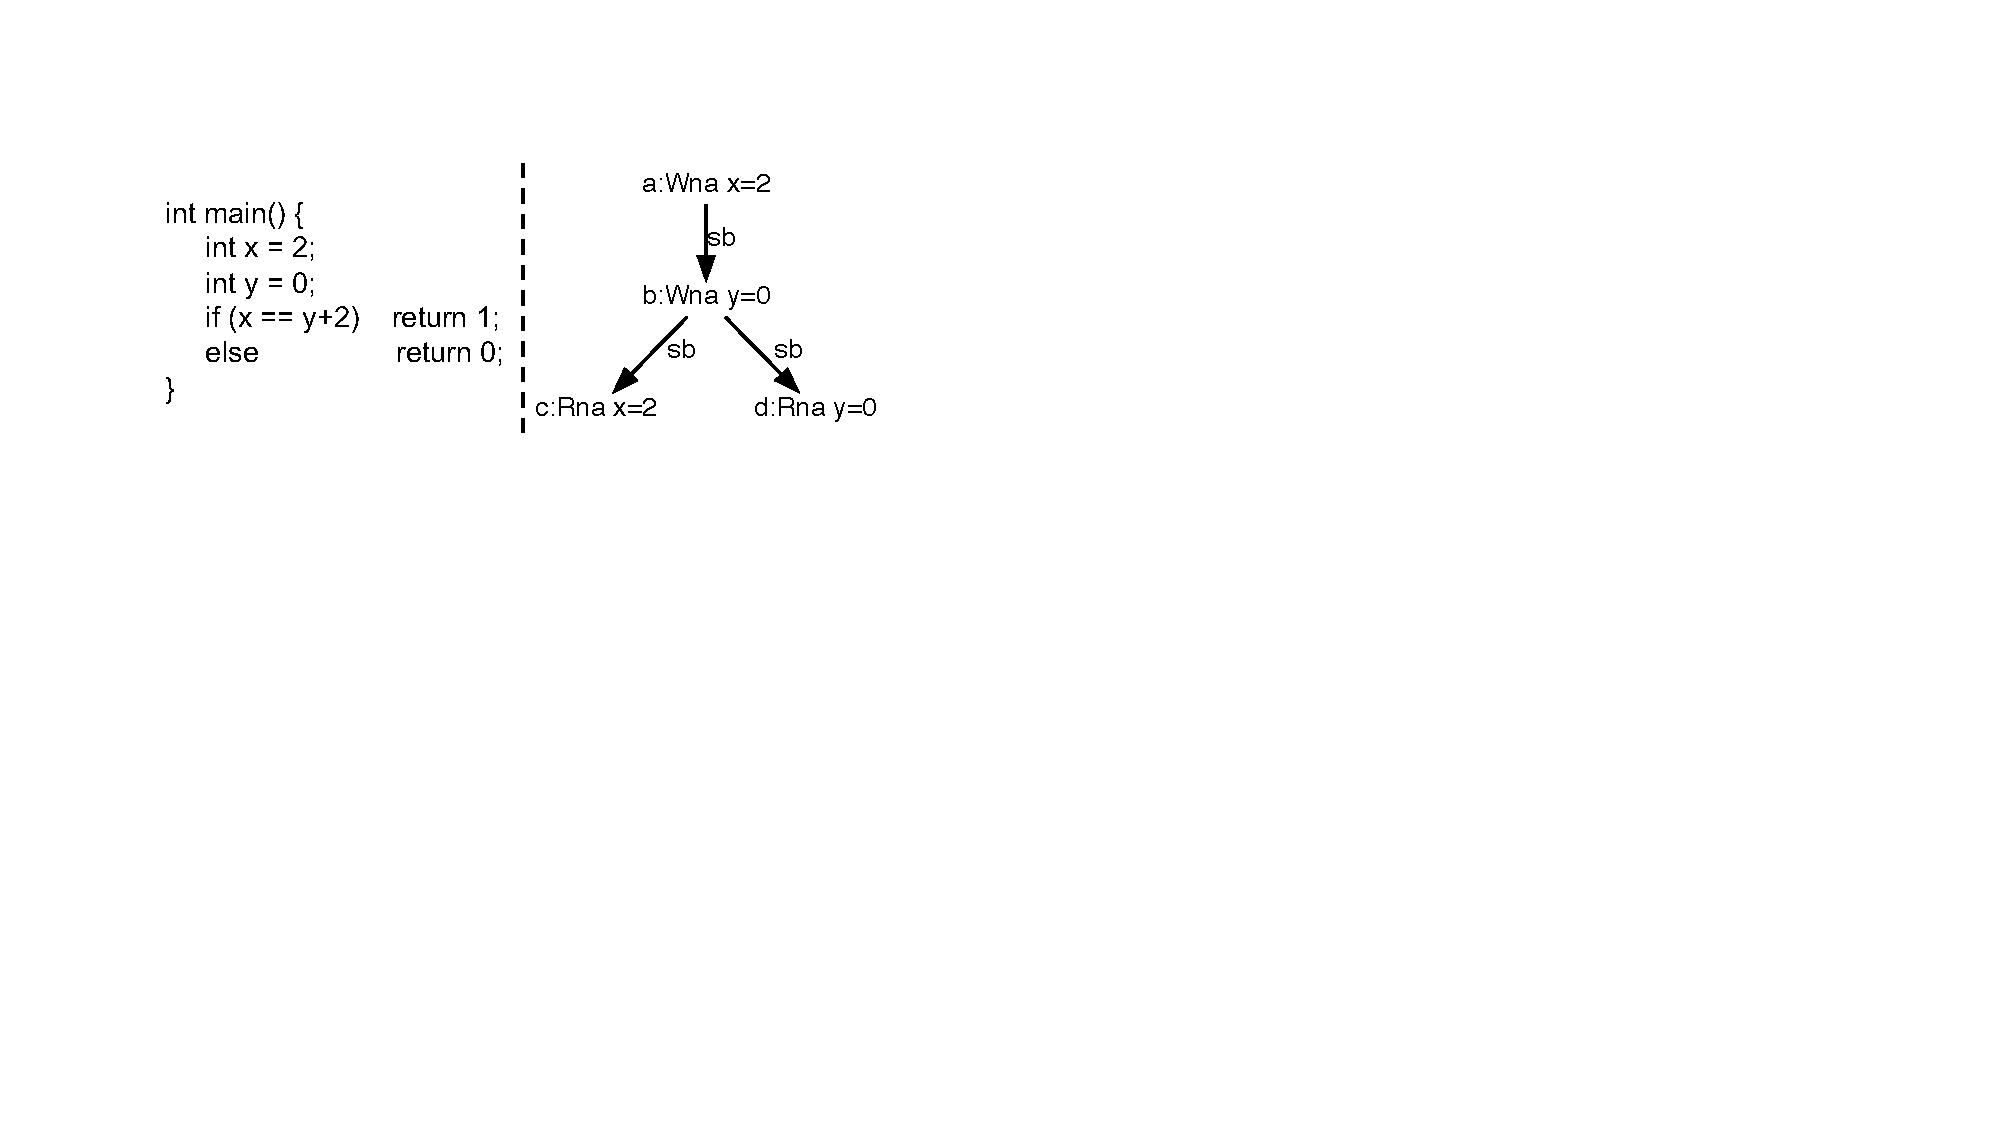
\includegraphics[scale=0.5]{sb_Relation.pdf} %[width=6in]
\caption{A simple example with one thread (on the left) and the \textit{sb}
relations among its actions (on the right).}
\label{fig:sb_relation}
\end{figure}

\paragraph{additional-synchronized-with}
The standard describes several situations that 
give rise to synchronization edges between actions. 
Apart from the main case described by synchronizes-with relation
(defined in Section~\ref{sec:relation3}), \textit{additional-synchronized-with} (\textit{asw}) 
describes all of the other cases. It mainly contains additional synchronization 
edges from thread creation and thread join among others.
Generally, synchronization edges order one part of program execution 
before another. Figure~\ref{fig:asw_relation} describes the \textit{asw} relations
for a simple example. 

\begin{figure}%[t]
\centering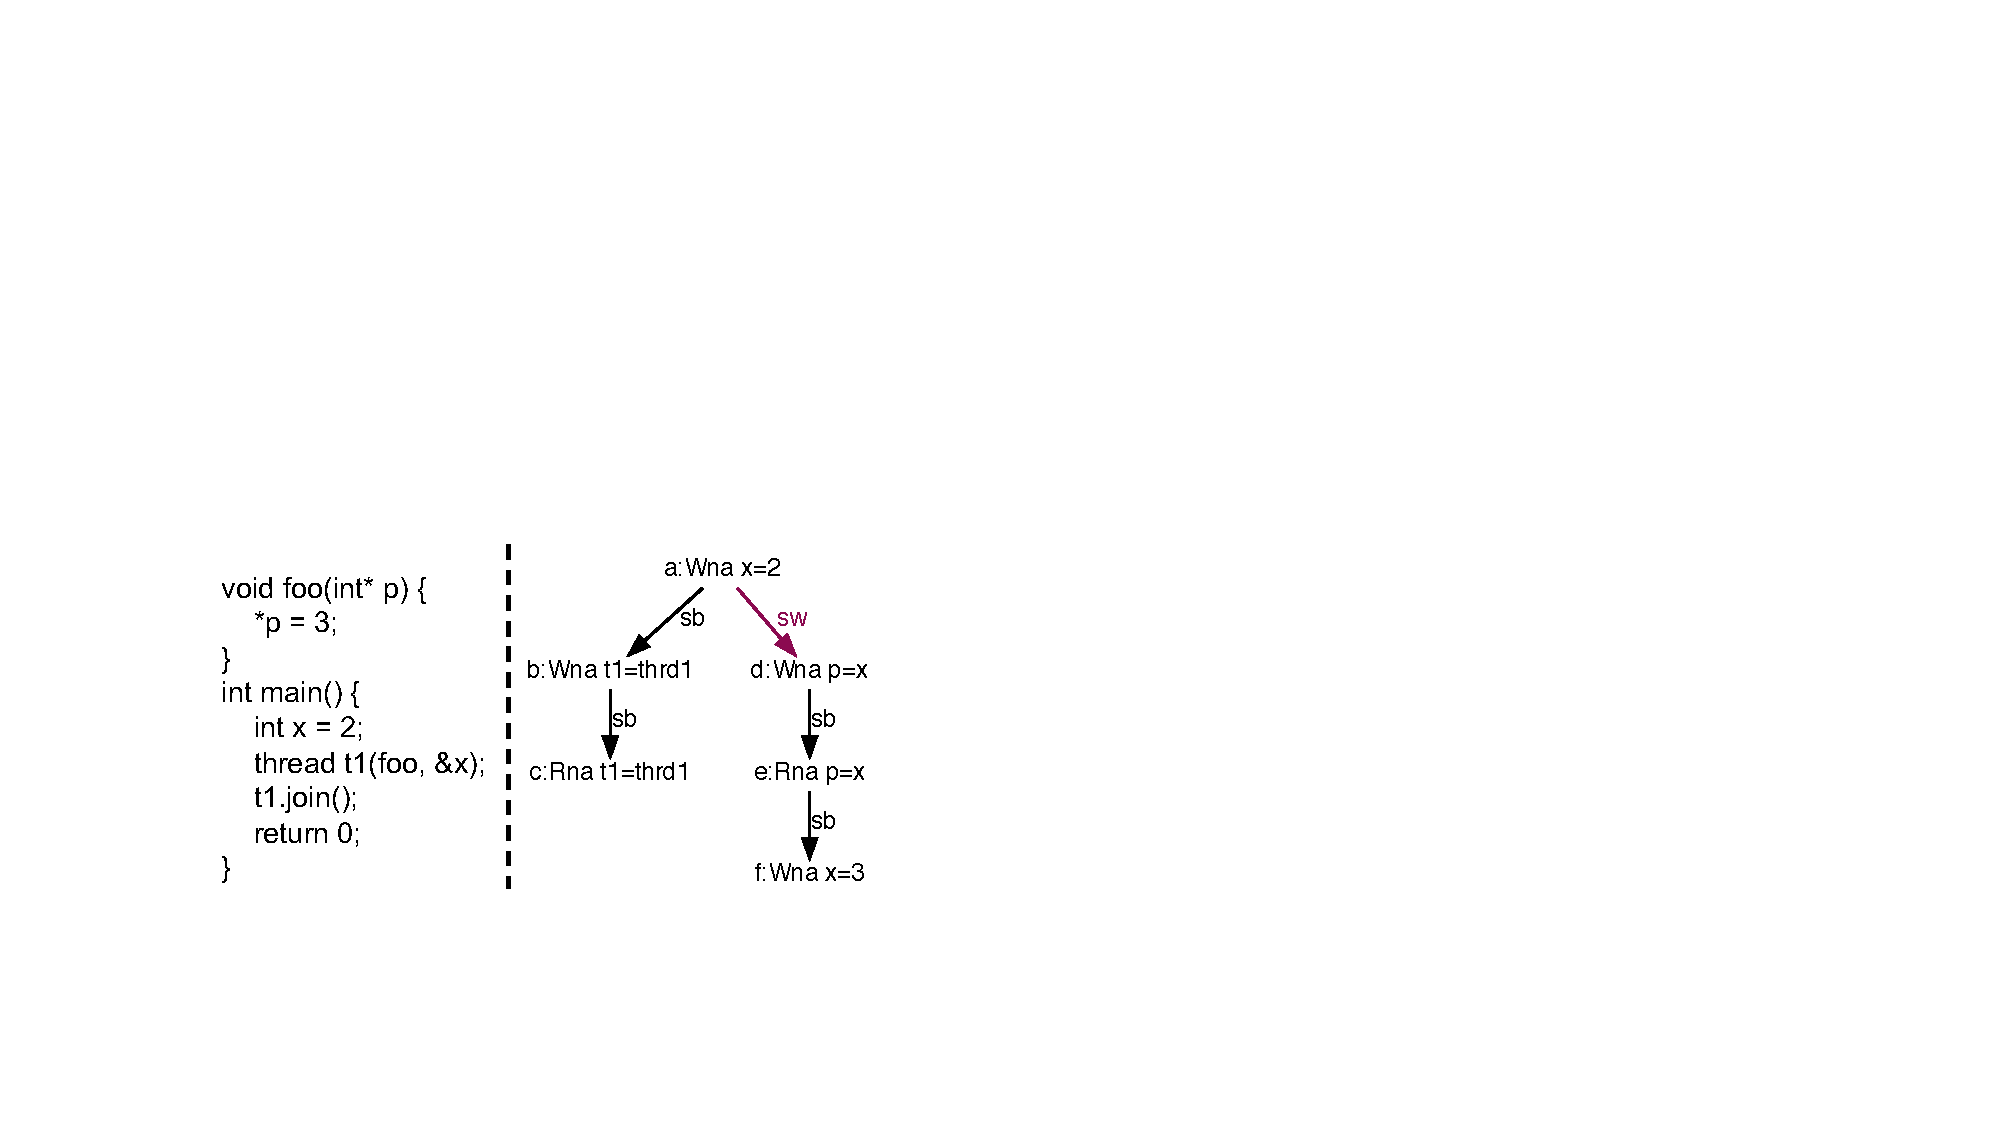
\includegraphics[scale=0.5]{asw_Relation.pdf} %[width=6in]
\caption{A simple example with two threads (on the left) and the \textit{sb} 
and \textit{asw} relations among its actions (on the right).}
\label{fig:asw_relation}
\end{figure}

\paragraph{pre-executions.}
Based on the two relations described above, 
\textit{pre-executions} can be defined as the program
executions which are compatible with the instructions of the individual 
threads without considering the behaviour of shared memory. 
In other words, a pre-execution is determined by \textit{sb} edges
and \textit{asw} edges.
Generally, \textit{pre-executions} are an over-approximation of the executions 
that will ultimately be allowed to happen once the whole program and 
the memory model are taken into account.

\subsubsection{Witness Relations}
\label{sec:relation2}

For each pre-execution, we can enumerate all its possible
\textit{candidate executions}, which comprise three more
relations: \textit{rf} (a reads-from map), modification-order (a coherence order), 
and \textit{sc} (an order over sequentially consistent actions). Specifically,
the added three relations are used to characterize the 
interrelationship between memory actions of different threads and thus
the behavior of a particular execution. Note that, not all 
pre-executions can be extended to a candidate execution. 
For example, a read cannot be matched with an expected write.

\paragraph{Reads-from}

This relation relates each write to every read that takes its value 
from that write. Note that the reads-from(rf) edges must relate writes 
and reads with the same value to guarantee a consistent execution. 
This relation is non-trivial, since in any given execution of a C++11 program, 
there are usually many stores that a load can read from. As described in
Figure~\ref{fig:rf_relation}, action \textit{c} is related to action \textit{d},
because \textit{d} reads the value written by \textit{c}. \textit{mo} and 
\textit{sc} edges will be described in the following section.  

\begin{figure}%[t]
\centering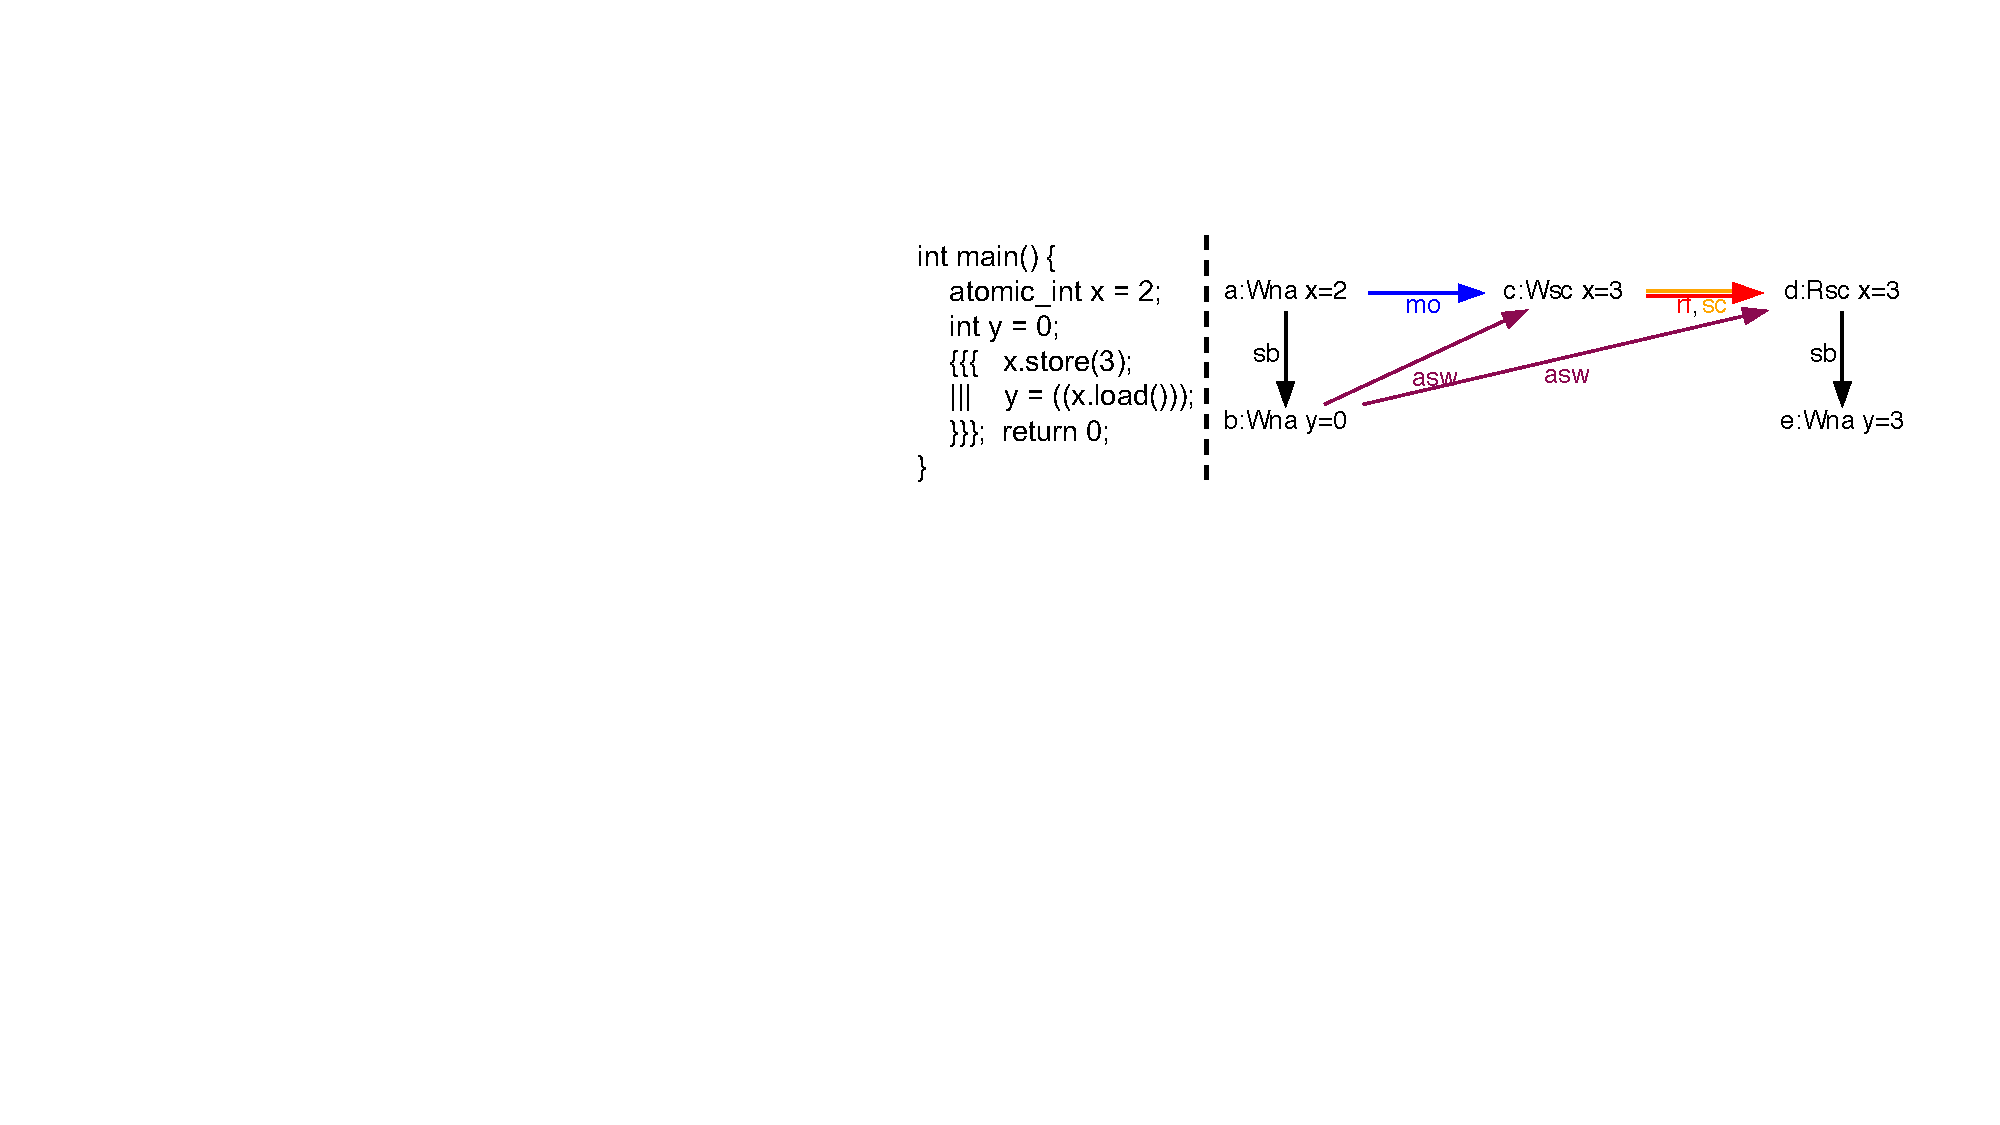
\includegraphics[scale=0.5]{rf_Relation.pdf} %[width=6in]
\caption{A simple example with three threads (on the left) and 
its three witness relations relations among its actions (on the right).}
\label{fig:rf_relation}
\end{figure}

\paragraph{Modification-order}

For each atomic location, a candidate execution has a total order 
of the writes to that location, and will be used to express coherence conditions. 
The union of all these relations 
is modification-order. This relation represents a memory-coherent
ordering in which the stores may be observed. 
Note that in general the modification orders for different objects 
cannot be combined to form a consistent total ordering, 
thus each location has its own order. As shown in Figure~\ref{fig:rf_relation},
the write actions \textit{a} and \textit{c} have a \textit{mo} relation with
\textit{mo} edge from \textit{a} to \textit{c}. 

\paragraph{Sequentially Consistent Order}

A program execution has a total order, \textit{sc}, over all 
of the atomic actions with sequentially consistent memory order 
and all of the lock and unlock actions of the program. 
This relation removes a lot of the weak behaviors that 
an execution could exhibit. 
For example, for a load \textit{a} and store \textit{b} both with 
sequentially consistent memory order, \textit{a} can not read from
\textit{b} when \textit{b} is prior to the most recent store in 
the \textit{sc} ordering. Taking Figure~\ref{fig:rf_relation} as 
an example, read \textit{d} cannot read from write \textit{a}, because
\textit{a} is pripr to \textit{c} which is in the same \textit{sc} ordering with \textit{d}. 


\subsubsection{Derived Relations}
\label{sec:relation3}

As described above, a candidate execution comprises its actions,
the relations determined by the syntax and control-flow, and 
the witness relations. To judge whether the execution follows 
the rules set out by the memory model and thus a consistent 
execution, several derived relations can be derived. 
These relations are completely determined by a candidate execution.

\paragraph{Release Sequence}

A release action is an atomic write or fence that has one of the 
three memory order: \textit{mo\_release}, \textit{mo\_acq\_rel},
and \textit{mo\_seq\_cst}. Each release write has a corresponding 
\textit{release sequence} (\textit{rs}), which is the longest continuous 
subsequence of the modification order that starts with the release
write, and each write in the sequence is performed by the same thread 
as the release or a atomic read-modify-write operations by any thread.
Note that the writes by other threads will break the sequence, however,
a RMW from another thread will continue it. Figure~\ref{fig:rs_relation}
describes one release sequence which is interrupted by a write action
from another thread. Note that the head of a release sequence has a 
\textit{rs} relation with itself.

\begin{figure}%[t]
\centering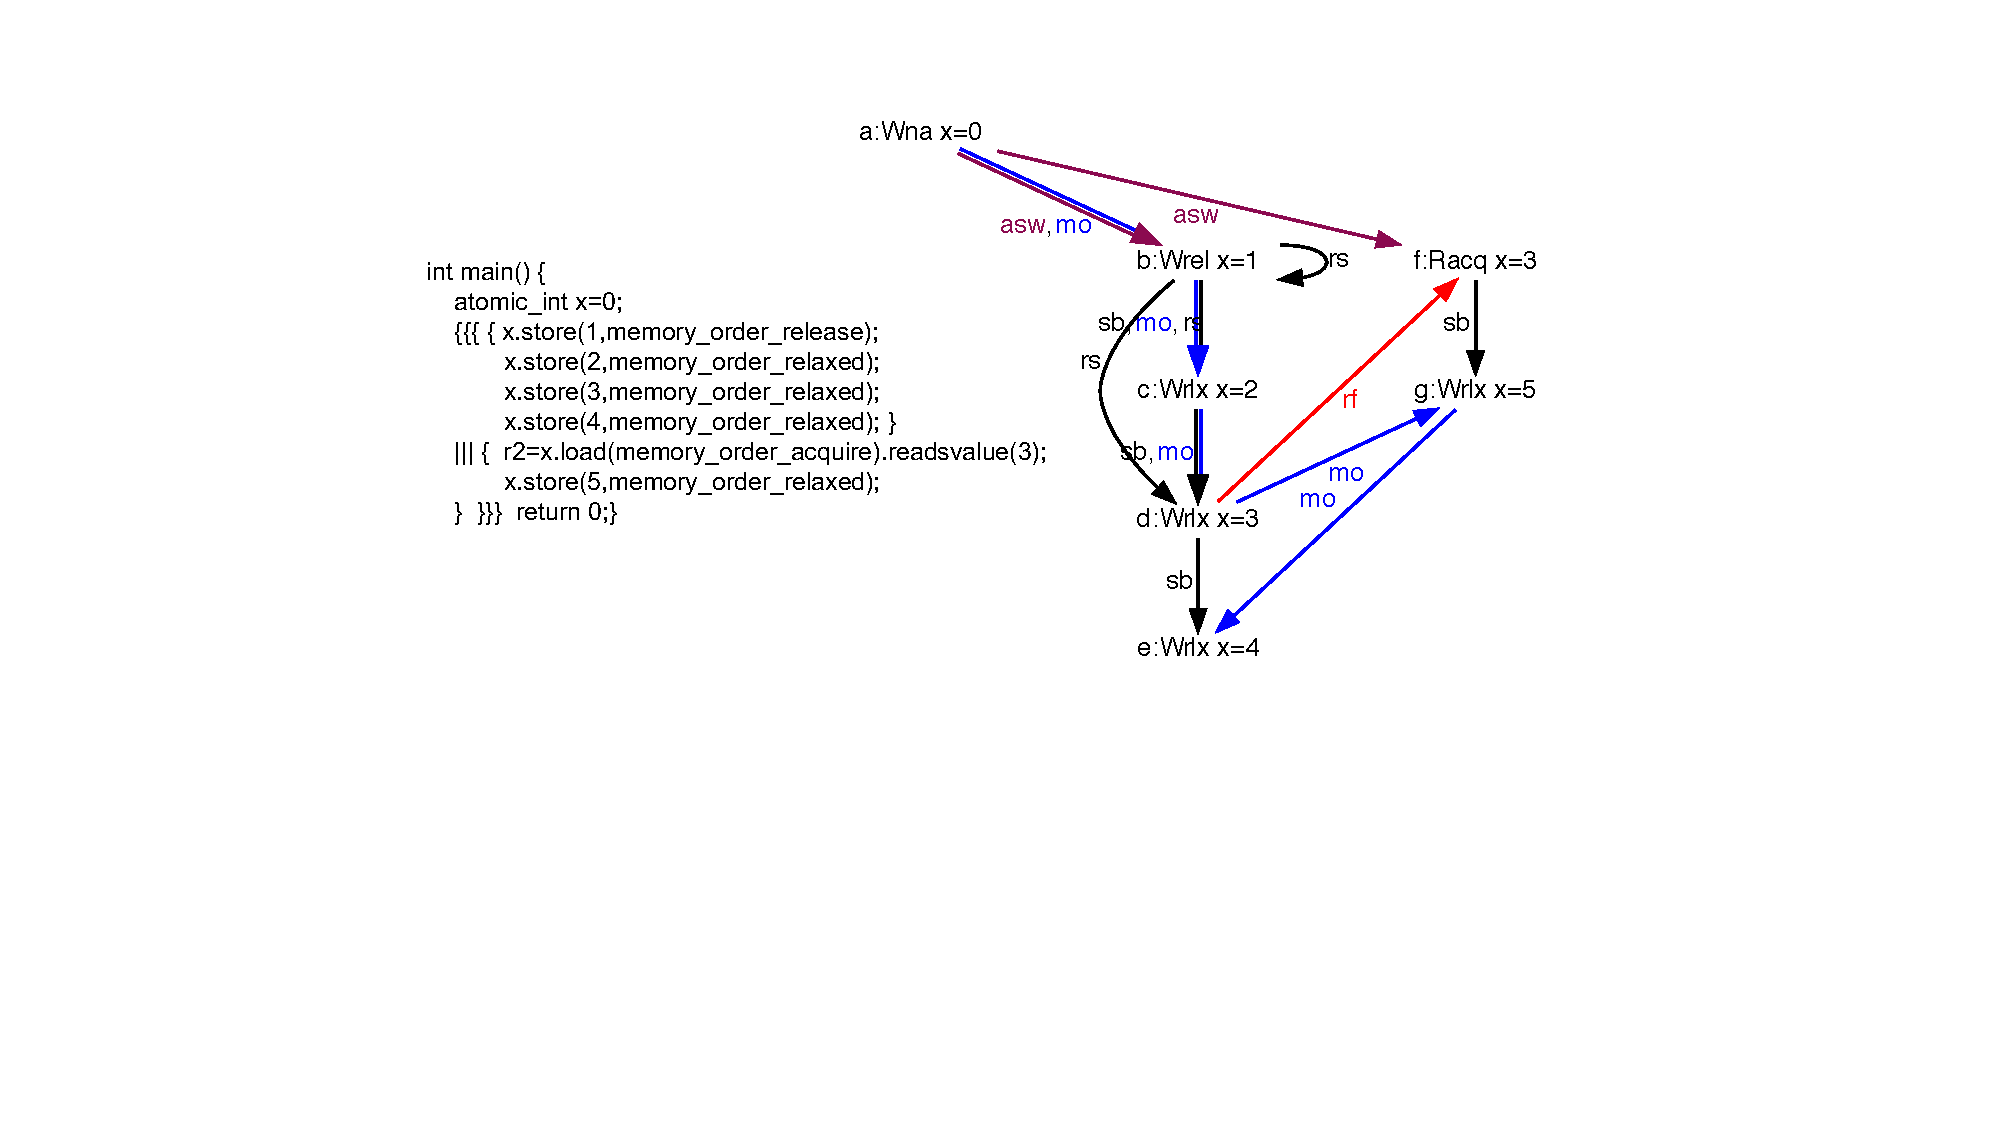
\includegraphics[scale=0.45]{rs_Relation.pdf} %[width=6in]
\caption{The release sequence begins at release action \textit{b}, and
ends at action \textit{d}. It contains three actions: 
\textit{b}, \textit{c}, and \textit{d}, and is interrupted by action \textit{g}.}
\label{fig:rs_relation}
\end{figure}

\paragraph{Hypothetical Release Sequence}

A hypothetical release sequence ($hrs$) is similar with a release sequence.
It has the same rules for extending and blocking as that for release sequences. 
The only difference is that a $hrs$ is headed by both release stores and non-release stores. 
The $hrs$ is used for describing fence synchronization.

\paragraph{Synchronizes-with}

This relation defines the points in an execution where
one thread has synchronised with another. 
An acquire action is an atomic read or fence that has 
either \textit{mo\_acquire}, \textit{mo\_acq\_rel}, \textit{mo\_seq\_cst} 
or \textit{mo\_consume} memory order. A release action synchronizes 
with an acquire action from another thread if the acquire action 
reads from a write in the \textit{release sequence} of the release. Then, 
a synchronizes-with (\texttt{sw}) edge exists between the acquire and 
release actions in the execution. 
This relation also occurs between consecutive unlock and lock 
operations on the same mutex, between thread creation and join.
Actually, an \textit{asw} edge is also an \textit{sw} edge.

\begin{figure}%[t]
\centering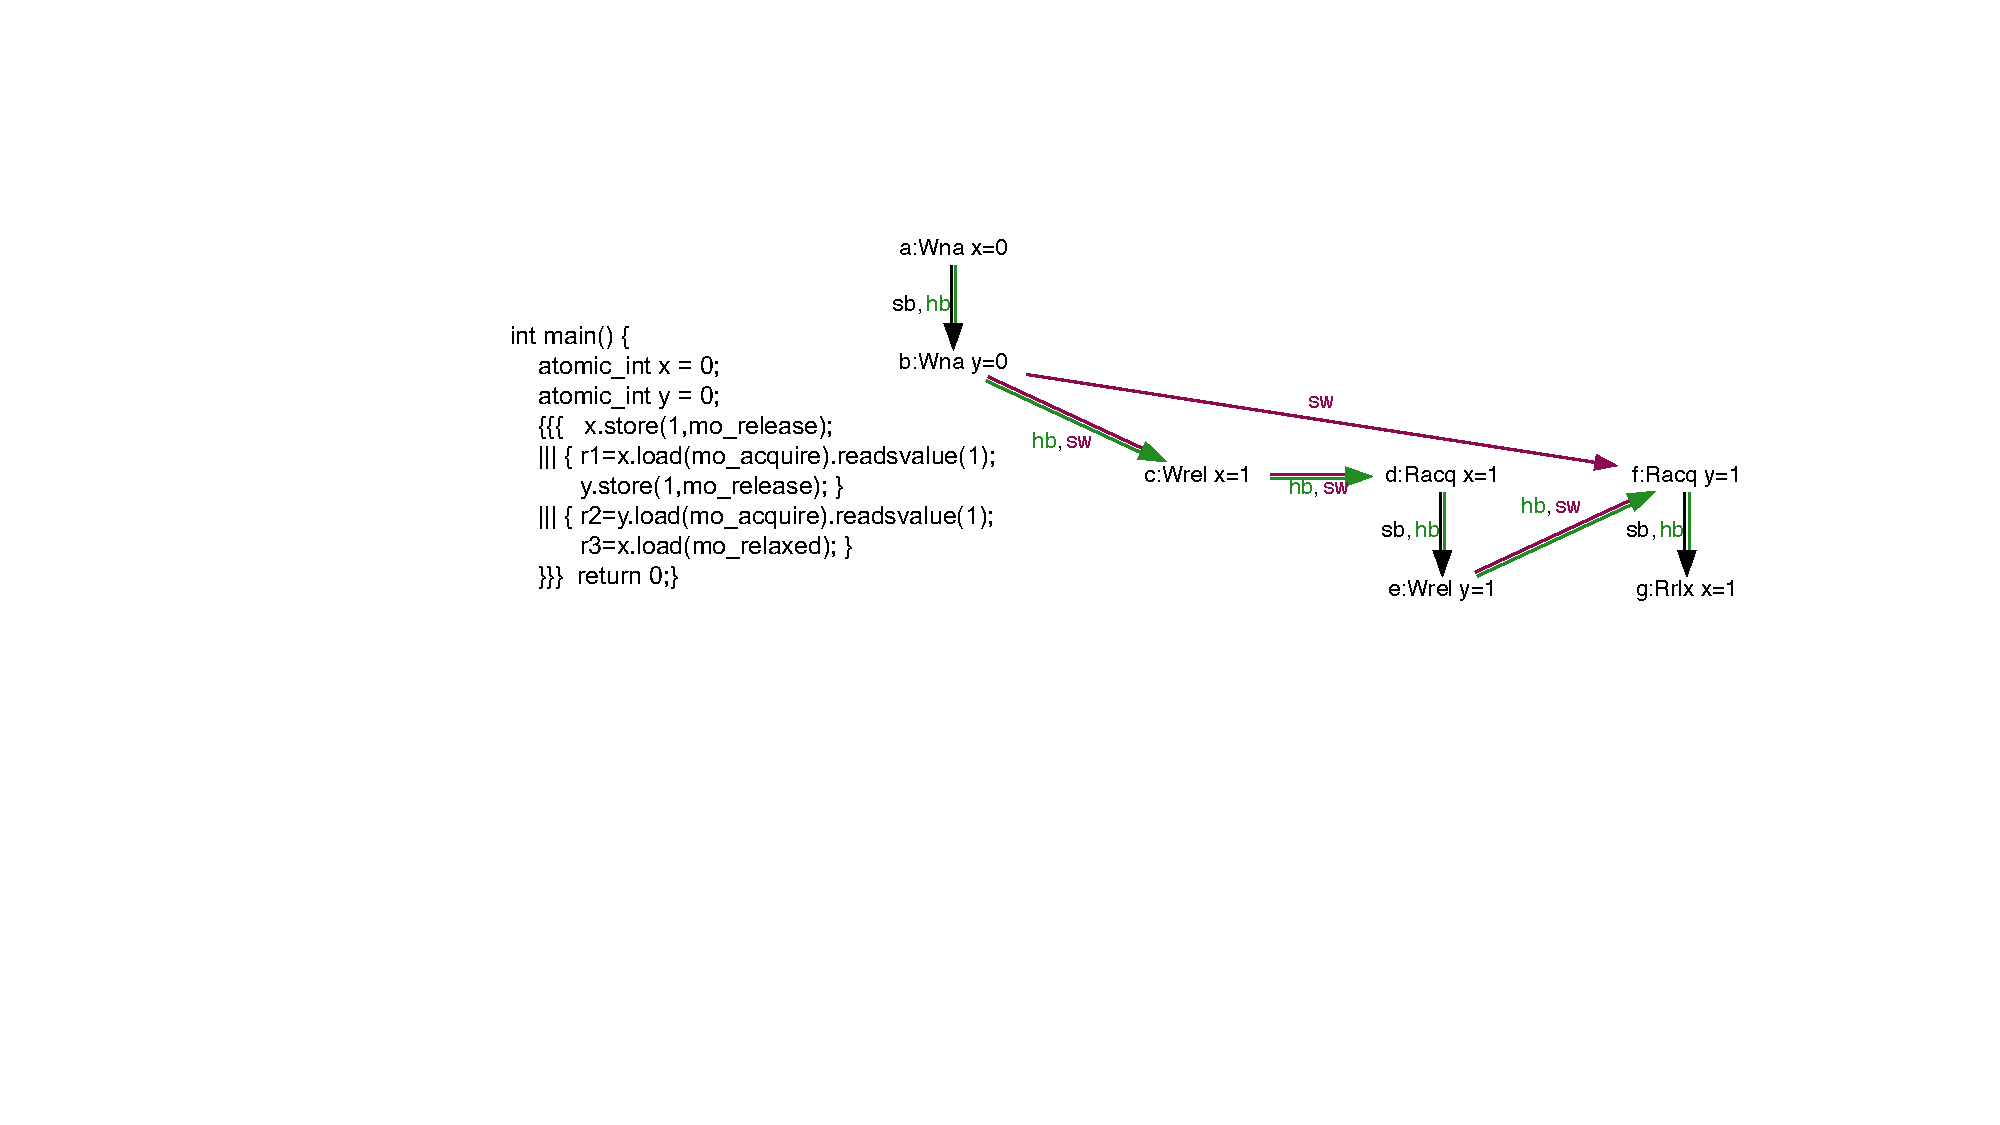
\includegraphics[scale=0.4]{sw_Relation.pdf} %[width=6in]
\caption{\textit{sw} edges generated from thread creates and 
release-acquire pairs. }
\label{fig:sw_relation}
\end{figure}

In Figure~\ref{fig:sw_relation}, the \textit{sw} edge from \textit{b} to \textit{c}
and from \textit{b} to \textit{f} are generated by thread creations. In addition,
the \textit{sw} edge from \textit{c} to \textit{d}, and that from \textit{e} to
\textit{f} are both generated by release-acquire pairs. 

\paragraph{Happens-before}

This is the main derived relation, which is an inter-thread relation 
collecting several ordering relations, discussed so far. 
Without considering memory order \textit{mo\_consume}, 
Happens-before (\textit{hb}) is defined as the transitive 
closure of \textit{sb} and \textit{sw}, represented as $(sb\cup sw)^+$. 
Note that, \textit{asw} is one special type of $sw$. 
As described in Figure~\ref{fig:sw_relation}, \textit{bf} edges is consistent
with \textit{sb} and \textit{sw} relations.  
%(where + denotes transitive closure).
% representing Lamport’s partial ordering over the actions in a system [25]. Because an sw edge is also an hb edge, when thread A synchronises with thread B, every side effect that has occurred inAup to this point will become visible to every action issued by B from this point.
%Data

%\paragraph{Visible-side-effect}
%
%In a consistent execution, the writes that can be read by a given read 
%are decided by the happens-before relation. Specifically, the writes that
%happens before the read with no intervening write is a\textit{ visible side effect} 
%of the read. For example, a write $A$ is visible with respect to a read $B$ if 
%$A$ happens before $B$, and no other write $X$ happens $B$ but after $A$. 
%For atomic reads, their visible side effects decide the earliest writes 
%in modification order that the reads may be read. 
%There can be at most one visible side effect for any load. 
%
%\paragraph{Visible-sequence-of-side-effects} 
%
%Atomic reads take their values from a write in a visible sequence of side effects of the read. This is a contiguous part of themodification order that starts with a visible side effect and ends before the first write that the read happens- before. In our diagrams of executions, we draw these sequences as vsses edges from their elements to the read that they correspond to (the order among the sequence is simply modification order). The following execution shows a read from a write in a visible- sequence-of-side-effects.


\subsection{Consistent Executions}
\label{sec:consistentExe}

Based on the currently defined relations, we can check whether a given 
candidate is a consistent execution. 
The C++11 memory model is axiomatic, and it provides a set of axioms 
to described an execution which may be exhibited by a program.
Only when a candidate execution conforms these axioms, then it is 
said to be consistent. Inconsistent executions need not to be taken into 
consideration, because they will never occur by any actual execution. 

Seven consistent axioms are proposed in~\citep{Batty:2011} to guarantee
the consistency of executions. 
The \textit{well\_formed\_threads} axiom requires that all actions are well-formed 
with expected memory orders and \textit{sb} must 
be intra-thread and a strict pre-order, an irreflexive and transitive order. 
The \textit{well\_formed\_rf\\\_mapping} axiom ensures \textit{rf} relation
enforces consistent behavior among different actions. For example, 
$a \stackrel{rf}{\longrightarrow} b$ implies that load \textit{b}
must read the value that a writes. 
The \textit{consistent\_locks} axiom states that the lock and unlock actions
at the same location is a strict total order, and it describes the similar
relation with that in C++ programs with sequential consistency memory model. 
The last three axioms, \textit{consistent\_sc\_order}, \textit{consistent\_mo} 
and \textit{consistent\_rf\_mapping}, correspond with the formation of the 
three derived relations: \textit{sc}, \textit{mo} and \textit{rf}. 
We do not consider \textit{consistent\_inter\_thread\_happens\_before}
relation with \textit{consume} operations, thus it simply requires \textit{hb} to 
be irreflexive. 

For thoroughly checking a C++11 program, we need to identify all the undefined
behaviors that may happen in a consistent execution. It is a tricky problem, since 
some weak behavior, not allowed by sequential consistent memory model,
can only happen with the effect of compiler reorderings and the hardware on 
which a program is executed. 

\section{Background...}
Add a simple introduction about maximal causality reduction and MCR. ...

\section{Our Approach}
\label{sec:approach}

Our approach, \checker, explores all consistent execution of a C++11 program allowed
by its memory model to identify abnormal behaviors based on
a constraint-solving method. Specifically, whenever a new execution is observed,
It identifies new unexplored consistent executions, and generates a corresponding schedule to
trigger each execution. 

In the following section, we first presents the main workflow in Section
~\ref{sec:workflow}, and describes the constraints encoding approach for 
consistent executions generation in Section~\ref{sec:encode}. 
Section~\ref{sec:check} describes the property checking along consistent executions, and 
Section~\ref{sec:identify} describes the identification of unexplored consistent executions. 

\subsection{The Main Workflow of \checker}
\label{sec:workflow}

Algorithm~\ref{alg:top} describes the main work flow of \checker. 
For a given C++11 program $P$, it firstly initializes the \textit{to-be-checked}
work list $workList$ with a random schedule $sch$, then it follows an
iteration process (line 4$\sim$11). For each iteration, it firstly gets an unexplored 
schedule $sch$ from $workList$ at line 5, and then carries out a concrete
execution to follow $sch$ at line 6. Line 7 constructs the constraints 
of maximal causal model (described in Section~\ref{sec:encode}), which will
be checked offline at line 8 (described in Section~\ref{sec:check}). 
At the end of each iteration, $workList$ will be updated at line 10 with newly
identified schedules based on the currently observed trace $\tau$ at line 9. 


\begin{algorithm}%[t]
  \caption{{\bf The main workflow of \checker.}}
%  its cycles as potential deadlocks.}}%: The top algorithm.
  \label{alg:top}
{%\footnotesize
\begin{algorithmic}[1]
  \State{\Ind{0} \textbf{Input:} C++11 Program $P$;}
%  \State{\Ind{0} \textbf{Output:} potential deadlocks $deadlocks$;}
  \State{\Ind{0} Let $sch$ be a random schedule;}
  \State{\Ind{0} $workList.add(sch)$;}
  \State{\Ind{0} {\bf while} ($workList\neq \emptyset$)}
  \State{\Ind{1} {		$sch\leftarrow workList.pop()$;}}
  \State{\Ind{1} {		$\tau\leftarrow$ \bf Execute$(P, sch)$;}}
  \State{\Ind{1} {		$\Phi\leftarrow$ \bf ConstructMaxCausalModel$(\tau)$;}}
  \State{\Ind{1} {		\bf PropertyCheck$(\Phi)$;}}
  \State{\Ind{1} {		$sch\_List\leftarrow$ \bf IdentifyNewSch$(\tau, \Phi)$;}}
  \State{\Ind{1} {		$workList.add(sch\_List)$;}}
  \State{\Ind{0} {\bf end while}}

\end{algorithmic}
}
\end{algorithm}

\subsection{Constraints Encoding of Maximal Causal Model}
\label{sec:encode}

As described in~\cite{Huang:2015}, while encoding the maximal causal model 
for the programs with sequential consistency memory model, only variables of 
the form $O_e$ corresponding to each even $e$ are needed. Specifically,
these variables denote the order of the actions in a given trace $\tau$. 
Unfortunately, such order variables are insufficient to describe the executions
for C++11 programs, since a strict total order does not exist among 
the actions from a given trace without the guarantee of sequential consistency 
memory model. Figure~\ref{fig:noStrictOrder} describes such an execution. 
%For example, even if two different memory locations are written 
%by the same thread in sequence, the two newly written values may be observed 
%in different order by other threads. 

\begin{figure}%[t]
\centering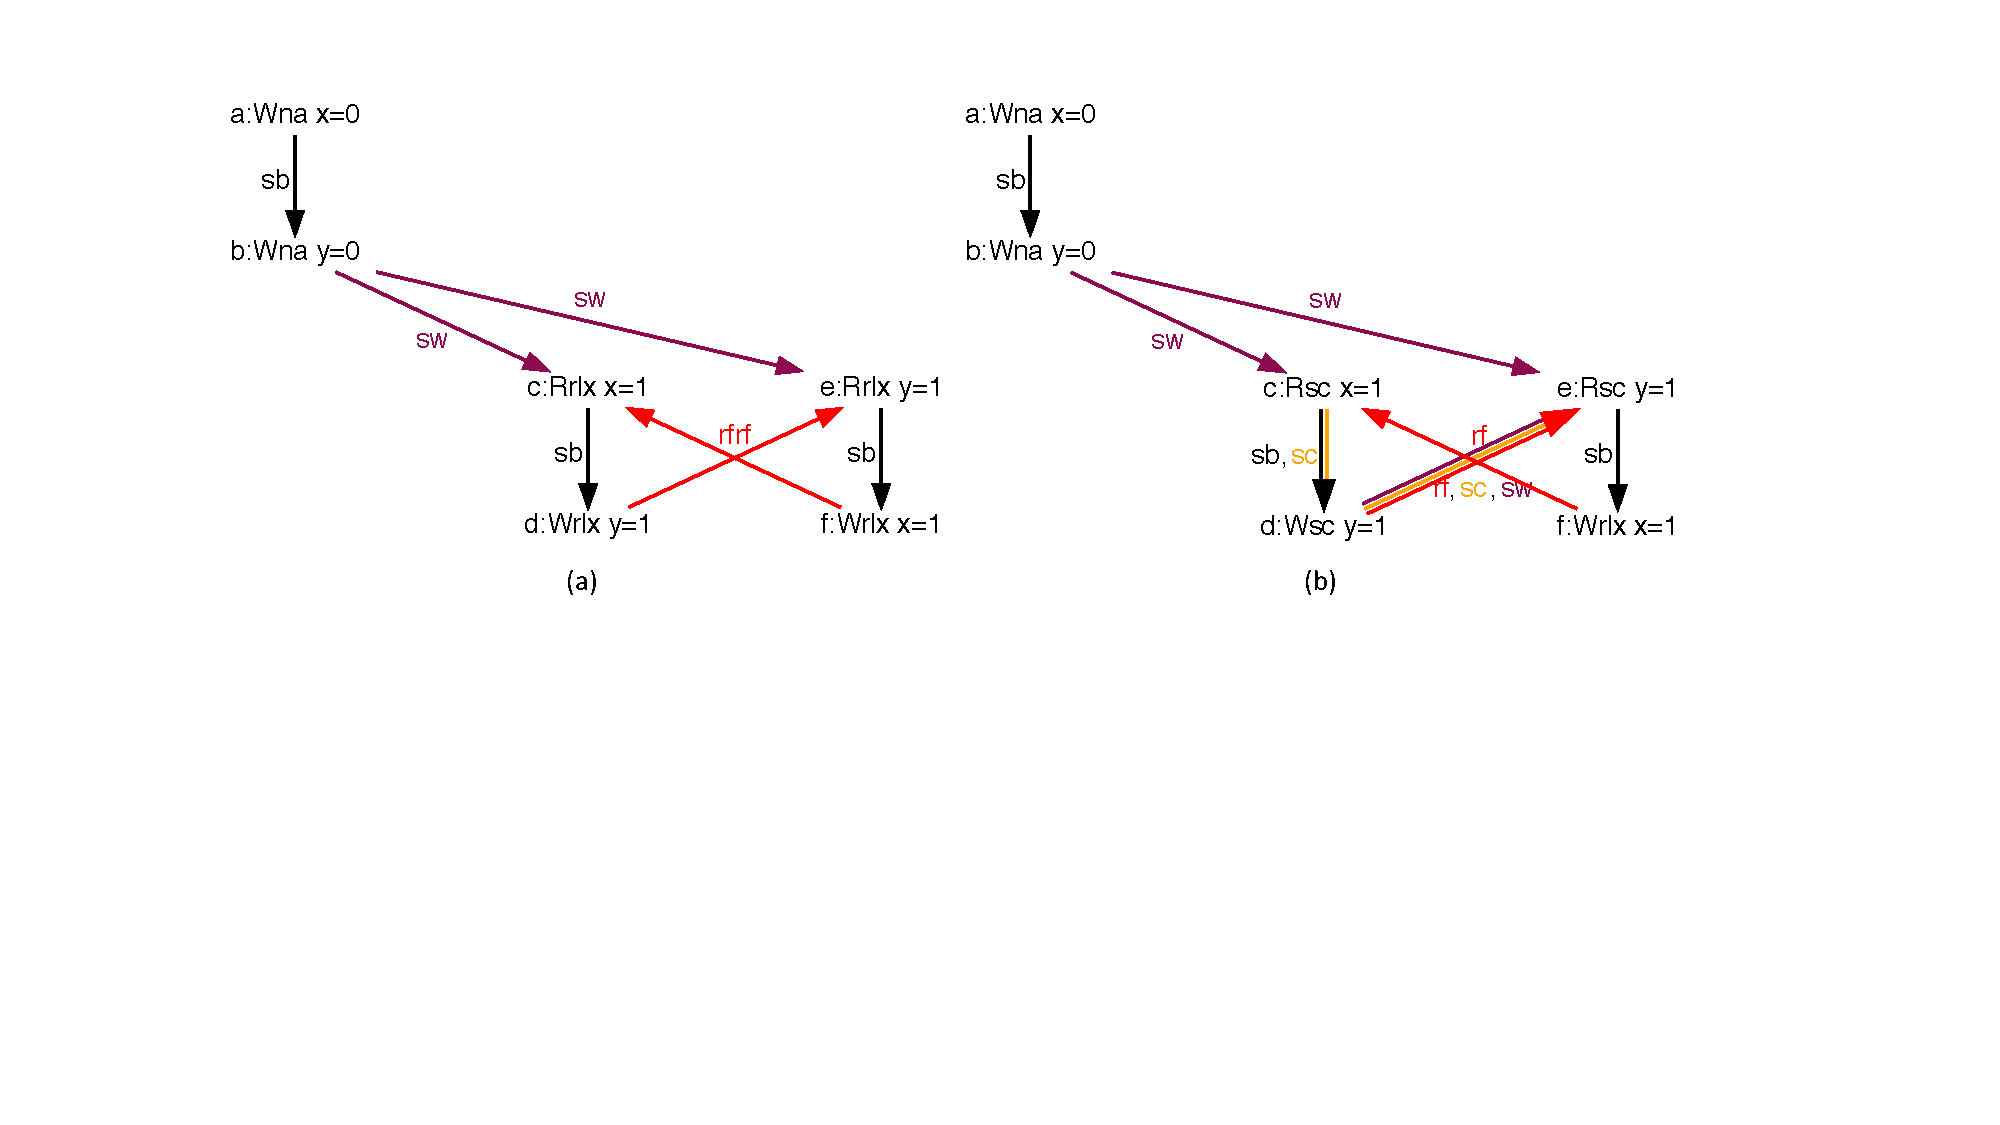
\includegraphics[scale=0.34]{noStrictOrder.pdf} %[width=6in]
\caption{(a) A consistent execution without a total order among
its actions. (b) An incosistent execution without any solution
on $\Phi$ because $\Phi_{corf}$ is violated. }
\label{fig:noStrictOrder}
\end{figure}

To describe the happens-before relation for the executions from C++11 programs, 
we use binary order variables $B$ among different actions.
Specifically, variable $B_{ab}$ represents the happens-before
relationship between action $a$ and $b$, which is set to 1 only when 
$a \stackrel{hb}{\longrightarrow} b$ and 
can be defined as follow: 

\[ B_{ab} = \left\{
  \begin{array}{l l}
    1,           &  {\text{if $a \stackrel{hb}{\longrightarrow} b$}};\\
    0,           &  {\text{if $b \stackrel{hb}{\longrightarrow} a$}};\\
    \bot,  &  \text{otherwise}.
  \end{array} \right.\]

Note that, instead of set $B_{ab}$ to 0, we always set $B_{ba}$ to 1 for simplification. 
Thus, in the following description, we only consider $B_{ab}$ if $B_{ba}=0$. 
Furthermore, $B_{ab}=\bot$ means that the action $a$ and $b$
have no happens-before relation, and thus can be executed \textit{concurrently}.   
%In addition, two other types of variables are used: $M$, $F$ and $S$.
%$M_{a}$ represents the memory modification order for a write $a$. 
%Note that, for each atomic location, the modification order for one location is a strict total order, but 
%it is incomparable among different locations. 
%$F_{ab}$ is another binary relation among a write $a$ and a read $b$, 
%and is set to 1 when $b$ reads from $w$, otherwise 0 is set. 

%\subsubsection{Constraint Encoding}

From a high level view, $\Phi$ can be encoded based on the variables $O$
(and three auxiliary types of variables: $M$, $F$ and $S$ described below), 
which denote the order of the actions in trace $\tau$. 
%According to the action relations described in Section~\ref{sec:relations}, 
Specifically, $\Phi$ is constructed by a 
conjunction of three sub-formulas: $\Phi\equiv\Phi_{hb}\wedge\Phi_{rw}\wedge\Phi_{co}$.
$\Phi_{hb}$ encodes the transitive happens-before relation, which contains both
must-happen-before relation and synchronizes-with relation. Specifically, we encode
the must-happen-before relation as $\Phi_{mhb}$, which encodes the \textit{sequence-before} 
relation and \textit{additional-synchronized-with} relation.
$\Phi_{rw}$ encodes the data-validity constraints, % enforced by the combined relations of $rf$, $mo$, and $sc$. 
and $\Phi_{co}$ encodes the coherence constraints. 

%conjunction of two sub-formulas: $\Phi\equiv \Phi_{1}\wedge \Phi_{2}$, where 
%$\Phi_1=\Phi_{sb}\wedge \Phi_{asw}$ represents the relations determined by syntax 
%and control-flow and $ \Phi_2 = \Phi_{rf}\wedge\Phi_{mo}\wedge\Phi_{sc}$ represents
%the witness relations. 

\subsubsection{must-happens-before relations $\Phi_{mhb}$}

We call the relations determined by syntax and control-flow must-happen-before relations,
which reflects a transitive closure relation of two union of relations: sequenced-before
relations ($sb$) and additional-synchronized-with relations ($asw$). 

The encode for $sb$ is straightforward, since $sb$ only 
considers the relations among the actions from the same thread, and 
we can generate the fact that $B_{ab}=1$ whenever 
$a$ and $b$ are actions from the same thread and $a \stackrel{sb}{\longrightarrow} b$. 
Note that when $b \stackrel{sb}{\longrightarrow} a$, we add a conjunct $B_{ba}=1$ instead of
$B_{ab}=0$. 

For encoding $asw$, we first identify all thread creation/join action pairs, $CJ$.
Specifically, each pair $(a,b)\in CJ$ describes the fact that the action $a$ in thread $T_i$ creates/joins to 
thread $T_j$ and the action $b$ is the first/last instruction of $T_j$. Thus,
$a$ must happens-before $b$ and $B_{ab}$ is set to 1.

Based on the encoded basic facts of both $sb$ and $asw$, we can encode $\Phi_{mhb}$ as follow: 

\begin{equation}
\begin{aligned}
\Phi_{mhb} = \bigwedge_{\forall a,b\in \tau} \Phi_{mhb}(a,b)
\end{aligned}
\end{equation}

where $\Phi_{mhb}(a,b)$ is defined as follow: 

\[\Phi_{mhb}(a,b) = \left\{
  \begin{array}{l l}
    B_{ab}==1,           &  {\text{if $a \stackrel{(sb\cup asw)^+}{\longrightarrow} b$;}}\\\\
    B_{ab}==\bot,  &  \text{otherwise}.
  \end{array} \right.\]

%At last, $\Phi_{mhb}$ can be described as the transitive closure of 
%the union of the definition of $sb$ and $asw$. 
When defining $\Phi_{mhb}$, '+' represents the computation of transitive closure. 
For the example in Figure~\ref{fig:noStrictOrder}, $\Phi_{mhb}$ will catch the relation
that $B_{ac}==1$. 

%\subsubsection{synchronizes-with relations $\Phi_{sw}$}
\subsubsection{Happens-before relations $\Phi_{hb}$}

Apart from the must-happen-before relation, C++11 programs 
contain three other types of synchronizes-with relations (the
mutex synchronization, release/acquire synchronization and fence synchronization),
which enforce the whole happens-before relation.  
%In this section, we mainly elaborate the encoding of release-acquire synchronization.

For mutex synchronization, it enforces the synchronizes-with relation among an unlock action $a$
and a lock action $b$ on the same lock $l$, if $a$ is ordered before $b$ in the sequentially consistent 
order $sc$.  Let variables $S$ represent the sequential orders for the atomic actions with sequential
memory order. For example, $S_a$ is the $sc$ order of the action $a$. Furthermore, 
let $Lock$ be the lock set, $L^l$ and $U^l$ respectively represent the lock/unlock action set on lock $l$. 
Then, for each pair of an unlock action $a\in U^l$ and a lock action $b\in L^l$ on the lock $l\in Lock$, the 
relation $a \stackrel{sw}{\longrightarrow} b$ exists only when $S_a<S_b$.

To describe the release-acquire synchronizations, we compute the release sequences
along $\tau$. %, represented as $rsSet$. 
Only when a acquire-read $r$ reads from one write $w$,
which belongs to the release sequence $Seq$ with release head $x$, the \textit{sw} edge 
$x \stackrel{sw}{\longrightarrow} r$ exists. Thus this relation can not be enforced 
as must-happen-before relation and directly encoded into $\Phi_{mhb}$. 
Let $acq(r)$ be $true$ only when action $r$ is a acquire-read,
%$rf^r_w$ be $true$ only when $r$ reads from $w$, 
$rsh(w)$ be the head of the release sequence which $w$ belongs to, 
$L$ be the set of the atomic locations and $W^x$ be the set of all the writes on location $x$. 
To describe the reads-from relation, we introduce the binary relation variables $F$ on each 
pair of a read and write action. Specifically, for a write action $a$ and a read action $b$, 
$F_{ab}$ is set to $true$ only when $b$ reads from $a$.
Then, for each pair of a read action $r\in R^x$ and write action $w\in W^x$ on location $x\in L$,
the relation $a \stackrel{sw}{\longrightarrow} b$ exists only when 
$acq(x)\wedge F_{wr}\wedge x\neq null$, where $x=rsh(w)$. 

\begin{figure}%[t]
\centering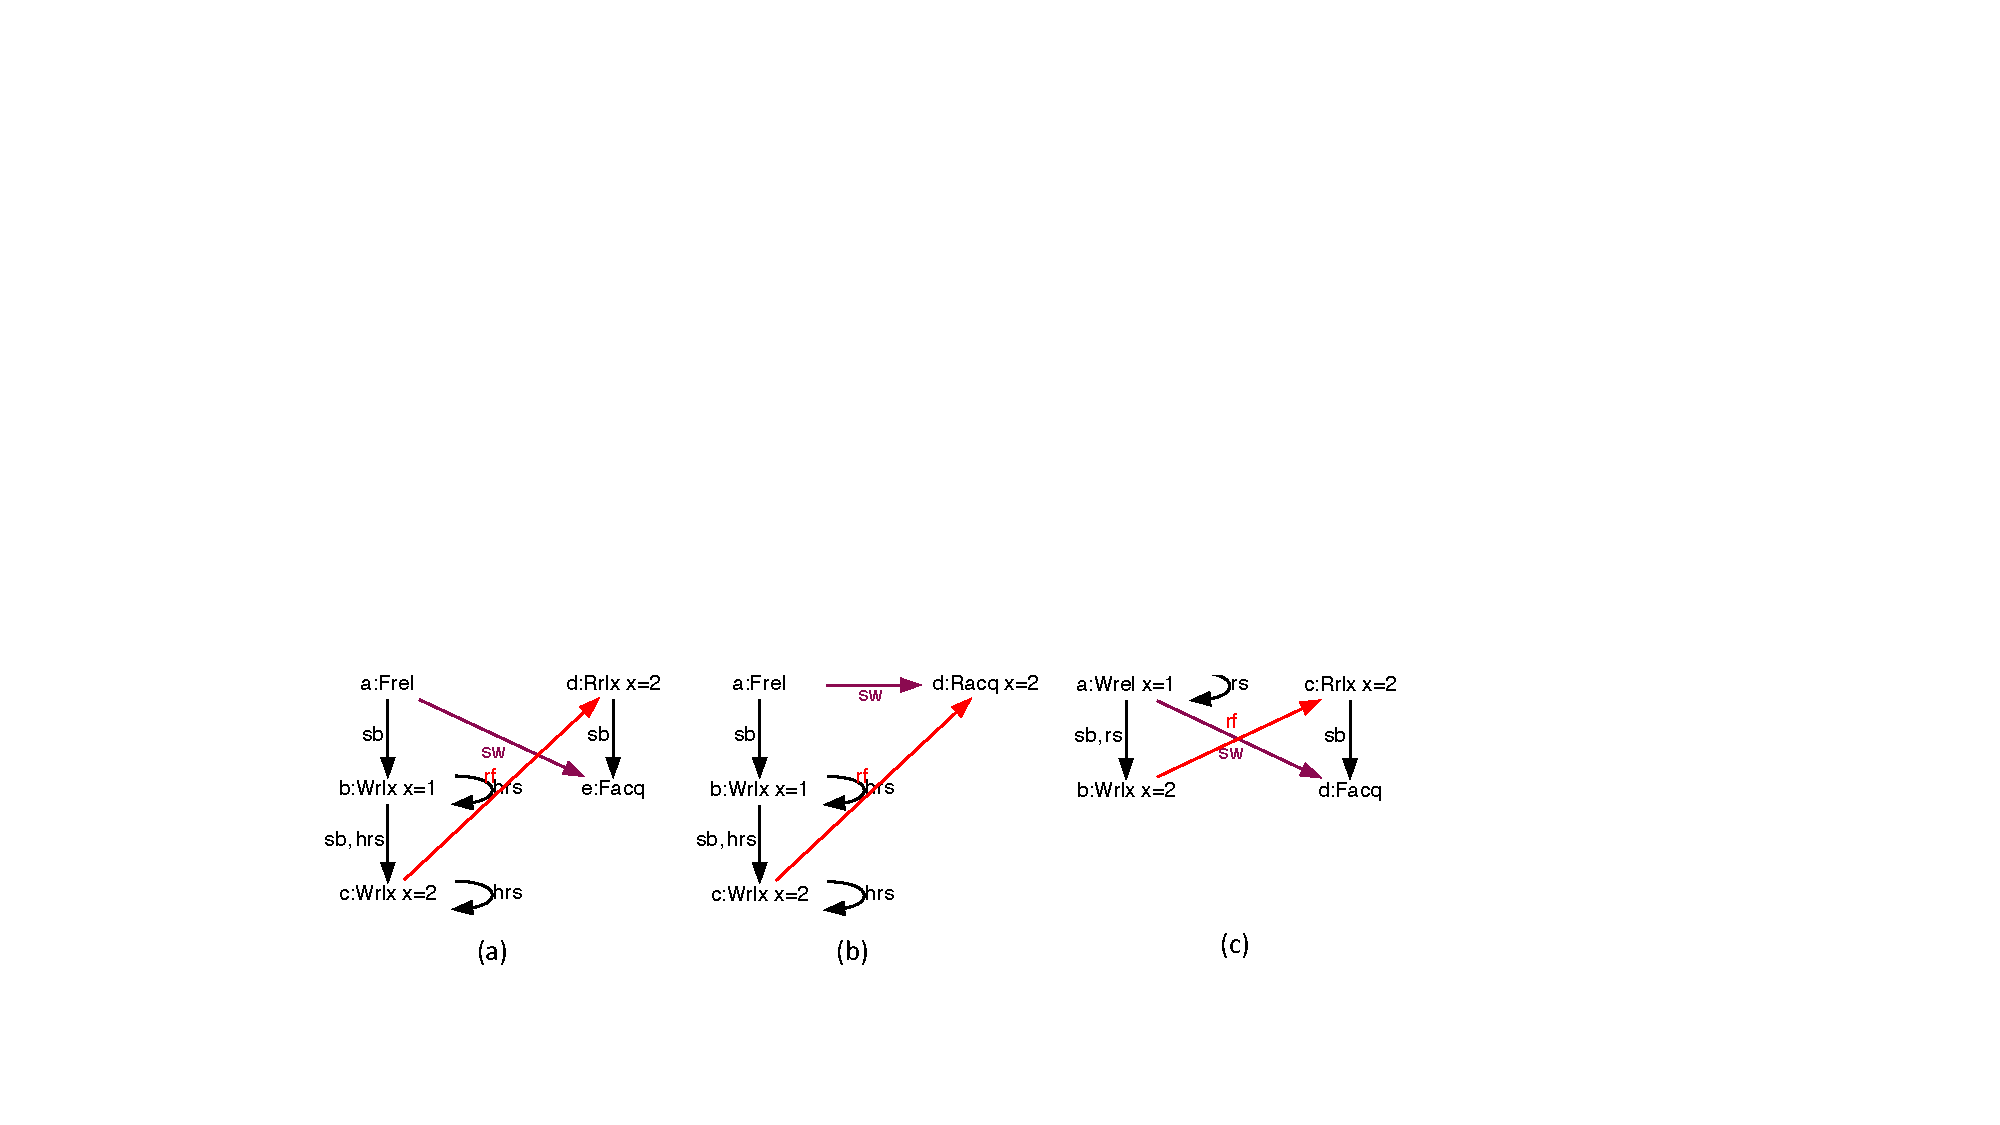
\includegraphics[scale=0.45]{fence.pdf} %[width=6in]
\caption{Three $sw$ relation types involved with fences. }
\label{fig:fence}
\end{figure}

Fences may also introduce synchronizes-with relations. Specifically, three types of $sw$ relation
are involved with fences, as described in Figure~\ref{fig:fence}. 
Specifically, Figure~\ref{fig:fence}(a) describes a $sw$ edge is enforced between a
release-acquire fence pair $(a,b)$ when there is a read $d$ reads from a write $c$, where
$a \stackrel{sb}{\longrightarrow} b$, $d \stackrel{sb}{\longrightarrow} e$ and 
$c$ is from the hypothetical release sequence of $b$. A release fence $a$ and an acquire read $d$
can also enforce a $sw$ edge, as described in Figure~\ref{fig:fence}(b), where $d$ reads from 
$c$, $a \stackrel{sb}{\longrightarrow} b$ and $c$ is a write from the hypothetical release sequence of $b$. 
The last case is described in Figure~\ref{fig:fence}(c). It describes a $sw$ edge enforced by a release 
write $a$ and an acquire fence $d$, when $c \stackrel{sb}{\longrightarrow} d$, $c \stackrel{rf}{\longrightarrow} b$
and $a \stackrel{sb}{\longrightarrow} b$.

The whole happens-before relation is a transitive closure of the union of the must-happen-before relation
and the synchronizes-with relation, thus we can encode $\Phi_{hb}$ as follow: 

\begin{equation}
\begin{aligned}
\Phi_{hb} = \bigwedge_{\forall a,b\in \tau} \Phi_{hb}(a,b)
\end{aligned}
\end{equation}

where $\Phi_{hb}(a,b)$ is defined as follow: 

\[ \Phi_{hb}(a,b) = \left\{
  \begin{array}{l l}
    B_{ab}==1,           &  {\text{if $a \stackrel{(mhb\cup sw)^+}{\longrightarrow} b$; }}\\\\
    B_{ab}==\bot,  &  \text{otherwise}.
  \end{array} \right.\]

\subsubsection{data-validity constraints $\Phi_{rw}$}

As described in~\cite{Huang:2015}, the data-validity constraints
ensure that every action in the considered trace $\tau$ is feasible. 
Specifically, to guarantee the feasibility of an action, we require that
all the actions that must-happen-before it should be feasible. Thus,
every read action that must-happen-before it should read the same value
as that in the input trace $\tau$.  

To describe all executions which exhibit the similar behavior as trace $\tau$, 
we do not require each read to read the value written by the exact same write action
as in trace $\tau$ but any possible write, as long as all required constraints
can be satisfied. For example, if more than one writes write the same value read
by a read action, then the read may read the value written by any write.  

Let $\Phi_{rw}(e)$ be the constraint of the reachability of the action $e$ in trace $\tau$,
then the data-validity constraint $\Phi_{rw}$
is a disjunction of the feasibility constraints of all actions in $\tau$, defined as follow:

\begin{equation}
\begin{aligned}
\Phi_{rw} = \bigvee_{\forall e\in \tau} (\Phi_{rw}(e))
\end{aligned}
\end{equation} 

The construction of $\Phi_{rw}(e)$ in sequential consistency memory model is straightforward,
it just requires that every read that must-happen-before $w$ should read 
the same value as that in the input trace. However, the \textit{happens-before} relation
in C/C++11 memory model dose not actually equals to the \textit{happen before} relation in sequential 
consistency memory model, thus such encoding will miss consistent executions for C/C++ programs with atomics. 
Furthermore, too loose constraint may result to inconsistency executions. 

\begin{figure}%[t]
\centering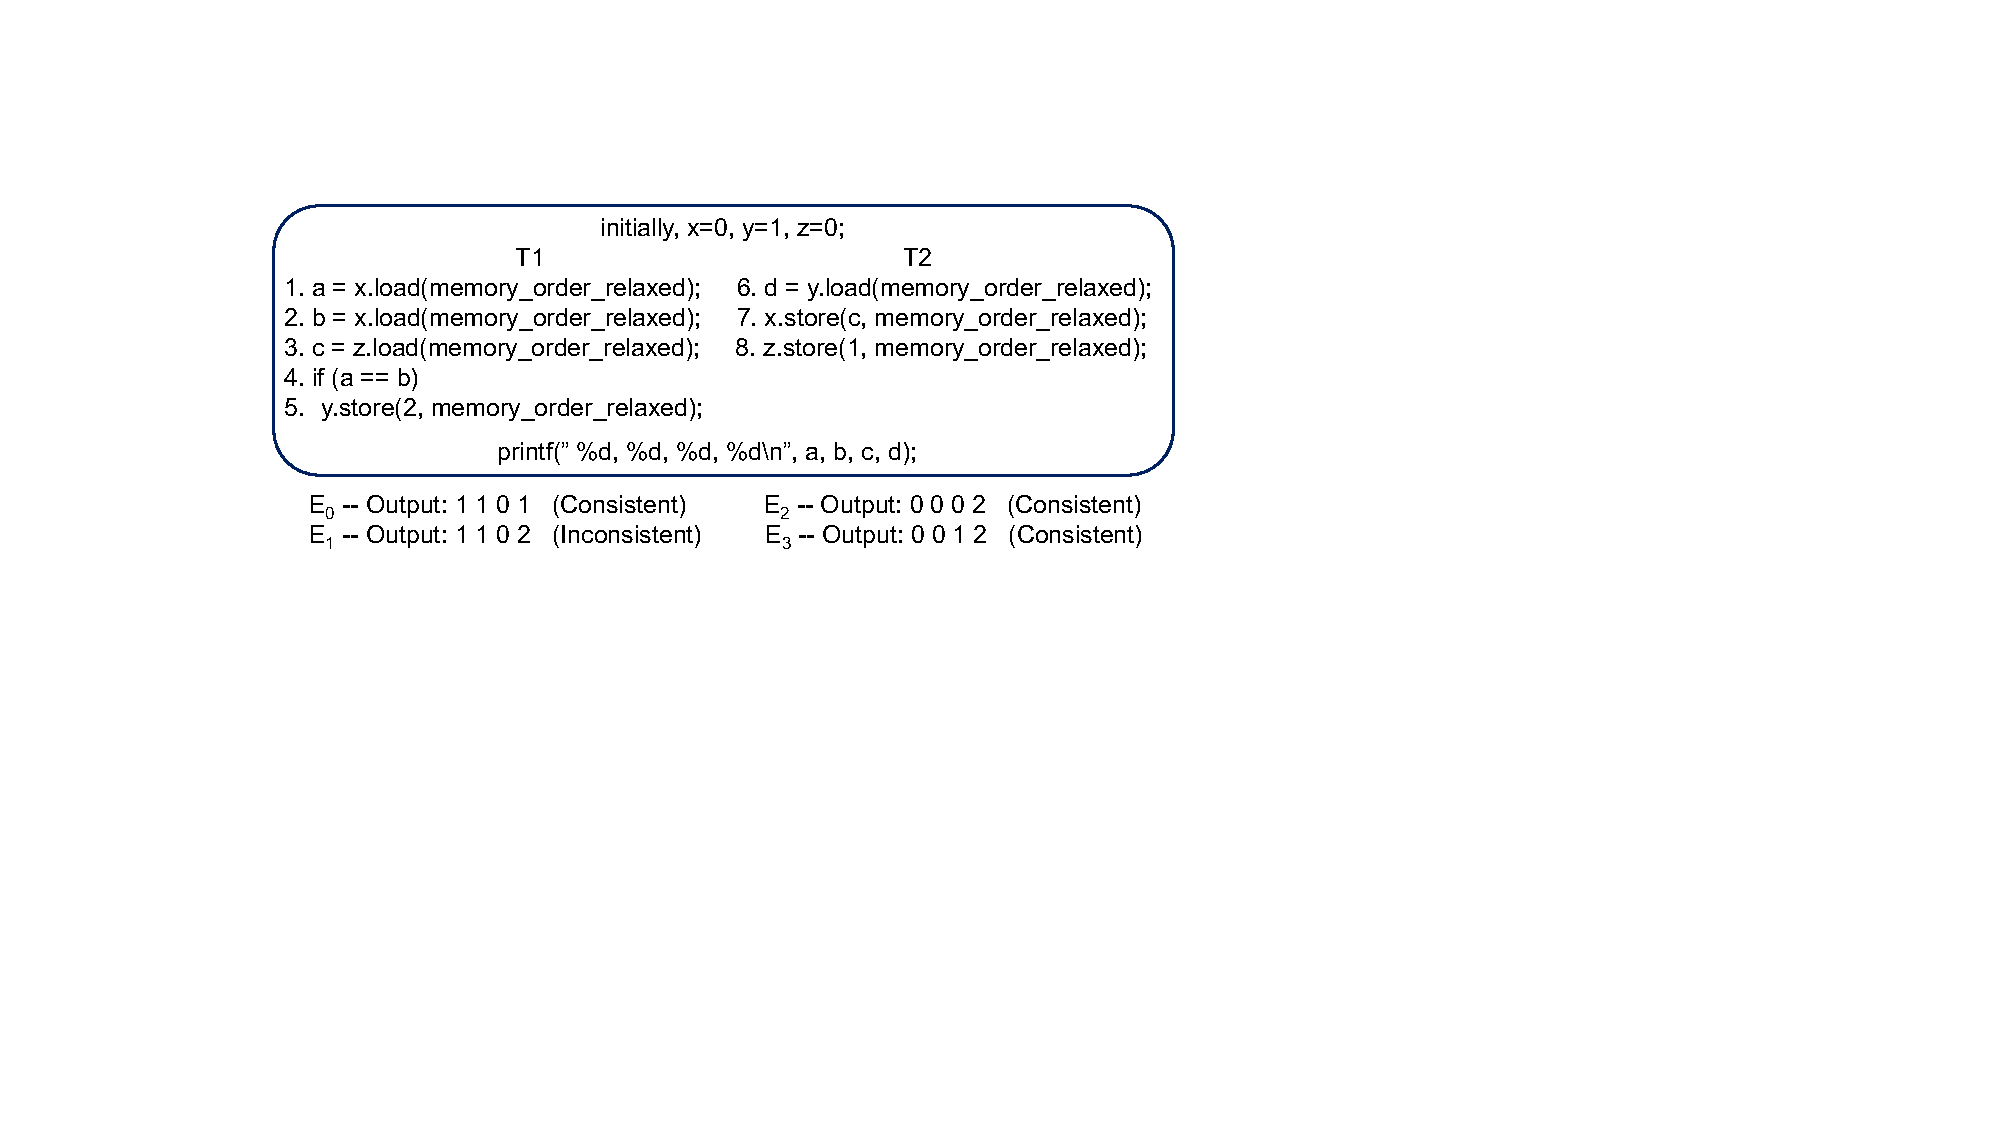
\includegraphics[scale=0.5]{inconsistency.pdf} %[width=6in]
\caption{Incorrect reachability constraints may introduce inconsistent executions or
miss consistent exectuions.}
\label{fig:inconsistency}
\end{figure}

Take the code snippet in Figure~\ref{fig:inconsistency} as example. 
$E_0$ is one of the possible consistent execution, based on which, 
we can generate a new schedule to enforce the execution $E_1$, 
when no reachability constraints is enforced. 
However, $E_1$ is actually an inconsistent execution which 
will not be manifested in the real world, 
since line 1 and 2 reads 1 requires that line 7 must store 1 to x,
thus $c$ loaded at line 6 must be 1, which is contradictory with the expectation that line 6 reads 2. 
Furthermore, the strict constraints which require that every read that must-happen-before 
$w$ read the same value as that in the input trace may miss some consistent execution. 
Let the input execution be $E_2$, then we can not identify the execution $E_3$ based on $E_2$,
since the reachability of line 5 requires that line 1, 2 and 3 all read 0.

To construct the appropriate reachability constraints, we carry out a dynamic control- and 
data-dependency analysis along each execution to identify the exact reads that an action 
really dependents on. Thus, we can successfully
identify the consistent execution $E_3$ based on $E_2$, because the reachability of the store at
line 5 only dependents on the read at line 1 and line 2, but not that at line 3.

Let $\stackrel{cd}{\longrightarrow} e$ be the set of the actions that 
the action $e$ control- or data-dependents on. 
For each read $r$ in set  $\stackrel{cd}{\longrightarrow} e$, $\Phi_{rw}(e)$
requires that $r$ must read the same value as that in $\tau$, represented as $value(r, \tau)$. 
%(\textit{Note that, we can not straightforward enforce all the reads that happens-before $e$,
%and we will explain the reachability problem in the next paragraph.})
Suppose %the set $W^x$ contains all the writes which write to location $x$, and 
the set $W_v^x\subseteq W^x$ contain these which write value $v$, then
$\Phi_{rw}(e)$ can be described as follow: 

\begin{equation}
\begin{aligned}
\Phi_{rw}(e) ={} & \bigwedge_{\forall r\in \stackrel{cd}{\longrightarrow} e} 
					(\Phi_{value}(r,value(r,\tau)))
\end{aligned}
\end{equation} 

where $\Phi_{value}(r,v)$ is defined as follow: 

\begin{equation}
\begin{aligned}
\Phi_{value}(r,v) ={} & \bigvee_{\forall w\in W_v^x} (\Phi_{rw}(w)\wedge F_{wr}\wedge 
					  B_{rw}\neq 1\wedge \\
					& (\bigwedge_{\forall w\neq w'\in W^x}\neg (B_{ww'}==1\wedge B_{w'r}==1)))
\end{aligned}
\end{equation}

The constraint $\Phi_{rw}(w)$ is utilized to guarantee the reachability of $w$. 
%requires that every read that must-happen-before 
%$e$ should read the same value as that in the input trace. 
The constraint $\Phi_{value}(r,v)$ enforces the read action $r=read(t ,x,v)$ 
to read the value $v$ on $x$ written by any write action $w =write(\_,x,v)$ in $W^x_v$.
Specifically, when the read $r$ reads the value written by the write $w$,
$w$ itself must be feasible, which is ensured by $\Phi_{rw}(w)$. 
%$\Phi_{sw}(r,w)$ is enforced to add the release-acquire synchronization, introduced by read-write pair $(r,w)$. 
$F_{wr}$ is enforced to require that the read $r$ reads the value written by the write $w$. 
Furthermore, it also subjects to the condition that $B_{rw}\neq 1$, which means that $r$ can
not happens before $w$. %Note that $B_{wr}\neq 0$ means $B_{wr}==1 \vee B_{wr}==\bot$.  
At the same time, there is no interfering write $w'$ between $w$ and $r$, represented as 
$\neg (B_{ww'}==1\wedge B_{w'r}==1)$, which means that 
$w'$ can not happens after $w$ but before $r$.
%Since not all the actions for C++11 programs can be sorted with 
%a strict total order, thus when two actions are incomparable, we need to enforce
%an order between them. 

\subsubsection{Encode coherence constraints $\Phi_{co}$}

As described in Section~\ref{sec:consistentExe}, seven consistent axioms should be 
enforced to ensure a consistent execution. We will not elaborate the first two axioms, 
\textit{well\_formed\_threads} and \textit{well\_formed\_rf\_mapping}, since they
are simple checks which are independent on any other relations. For example, 
\textit{well\_for\\med\_threads} requires that each atomic action should have a correct
memory order. \textit{well\_formed\_rf\_mapping} require that \textit{rf} relation must related a write and 
a load to the same location. The following section will respectively consider three axioms:
\textit{consistent\_sc\_order}, \textit{consistent\_mo} and \textit{consistent\_rf\_mapping}.
Furthermore, $\Phi_{co}$ is encoded as $\Phi_{co}=\Phi_{sc}\wedge\Phi_{mo}\wedge\Phi_{rf}$. 

\paragraph{Sequential consistent order $\Phi_{sc}$}

It enforces a total order over all the atomic actions with sequential memory order and 
all lock/unlock actions, denoted by the set $SC$. 
For consistency, the happens-before relation and modification order relation among the actions
in $SC$ should be restricted to the \textit{sc} order. 
%For each action $a$ in $SC$, we use $S_a$ to represent its sequential order, based on
$\Phi_{sc}$ can be encoded as follow: 

\begin{equation}
\begin{aligned}
\Phi_{sc} = (\bigwedge_{\forall a,b\in SC}(B_{ab}\neq \bot)\wedge (B_{ab}==1\rightarrow S_a<S_b)) \\
                   \bigwedge (\bigwedge_{\forall x\in L}\bigwedge_{\forall a,b\in W^x} (M_a<M_b\rightarrow S_a<S_b))
\end{aligned}
\end{equation} 

Note that $B_{ab}\neq \bot$ is used to enforce a total order among the actions
in $SC$. 


\paragraph{Consistent modification order $\Phi_{mo}$}

The modification order is a strict total order over the writes to the same location, thus 
the happens-before relation should be restricted to the modification order relation 
at the same location. $\Phi_{mo}$ can be defined as follow: 

\begin{equation}
\begin{aligned}
\Phi_{mo} = \bigwedge_{\forall x\in L }\bigwedge_{\forall a,b\in W^x} ((B_{ab}==1\rightarrow M_a<M_b) 
\end{aligned}
\end{equation} 


\paragraph{Consistent reads from mapping $\Phi_{rf}$}

\begin{figure*}%[t]
\centering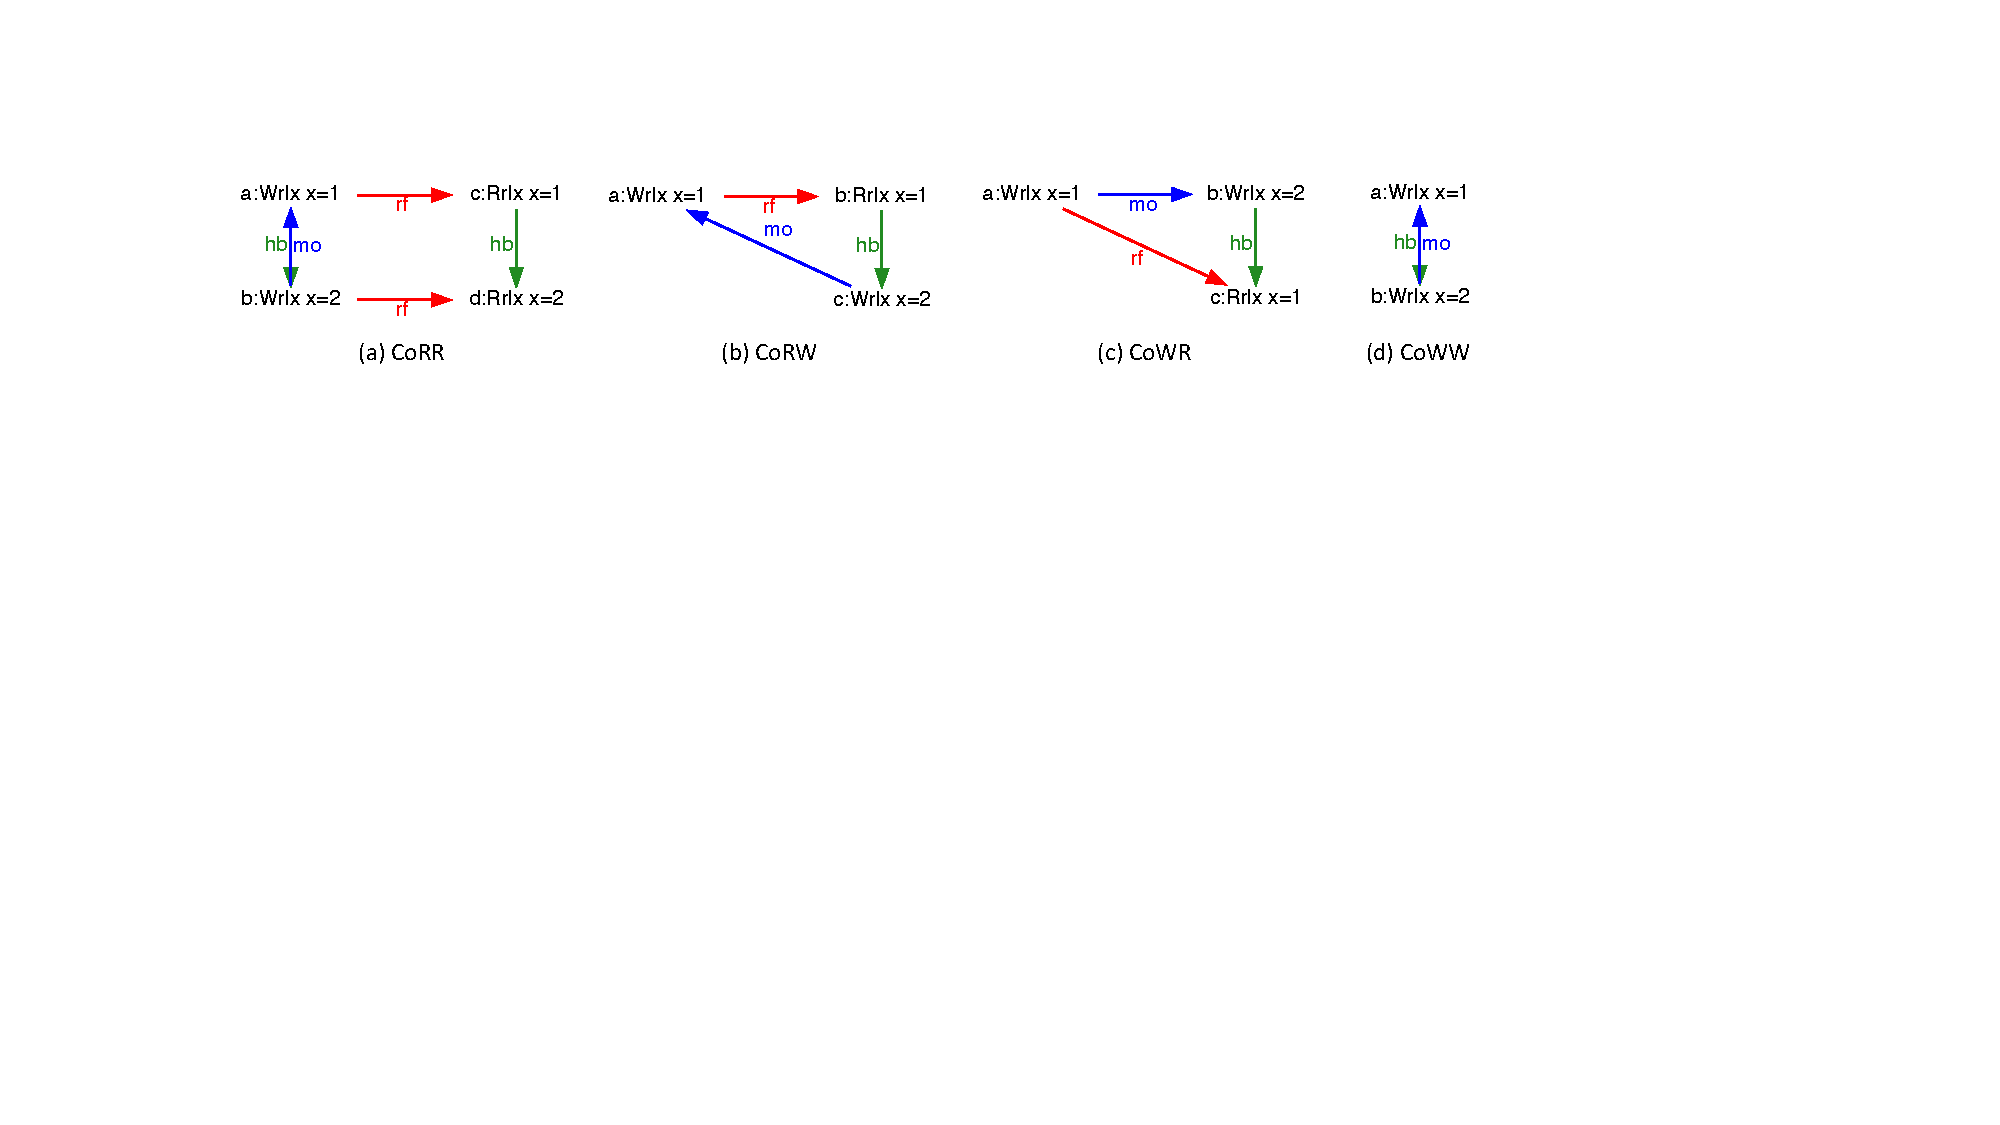
\includegraphics[scale=0.65]{CO.pdf} %[width=6in]
\caption{Four types of coherence restrictions.}
\label{fig:CO}
\end{figure*}

Memory model makes the key restriction on the values that memory actions can read. 
For each location, four types of coherence restrictions 
(CoRR, CoRW, CoWR, CoWW) are applied to the 
values that a read action can read. Each restriction explains the forbidden behavior of 
an execution. Figure~\ref{fig:CO} describes four forbidden example executions enforced
by each restriction. 

Let variable set $M$ be the memory modification order for an atomic write. For example, 
$M_{a}$ represents the memory modification order for a write $a$. 
Note that, for each atomic location, the modification order for one location is a strict total order, but 
it is incomparable among different locations. 

$\Phi_{rf}$ can be constructed by the conjunction of five
types of restrictions as $\Phi_{rf}=\Phi_{corf}\wedge\Phi_{corr}\wedge \Phi_{corw}
\wedge\Phi_{cowr}\wedge\Phi_{coww}$. The first conjunct $\Phi_{corf}$ restricts that each $rf$ relation
is consistent and is described as follow: 

\begin{equation}
\begin{aligned}
\Phi_{corf} = \bigwedge_{\forall x\in L }\bigwedge_{\forall a\in W^x, b\in R^x} ((F_{ab}\rightarrow B_{ba}\neq 1) 
\end{aligned}
\end{equation} 

$\Phi_{corf}$ enforces that when a read $b$ reads from a write $a$, 
then $b$ can not happens-before $a$. 
%Specifically,$R^x$ be the set of all the reads on location $x$. 

\textbf{CoRR} forbids two reads with happens-before relation (such as two reads
in a single thread) from observing two writes in an order inconsistent with modification order. 
To forbid such inconsistent executions as described in Figure~\ref{fig:CO}(a), 
we encode $\Phi_{corr}$ as follow: 

\begin{equation}
\begin{aligned}
\Phi_{corr} = \bigwedge_{\forall x\in L}(\bigwedge_{\substack{\forall a,b\in W^x\\c,d\in R^x}} 
(F_{ac}\wedge F_{bd}\wedge B_{cd}==1) \\
\rightarrow M_{a}<M_{b})
\end{aligned}
\end{equation} 

\textbf{CoRW} requires that a read that is happens-before a 
write should not be able to read from a later write in modification order.
As described in Figure~\ref{fig:CO}(b), the read $b$ can not read from
the write $a$, because $b$ happens-before $c$ and $a$ is a later write 
with $c$ in the modification order. To forbid such inconsistent executions, we 
encode $\Phi_{corw}$ as follow: 

\begin{equation}
\begin{aligned}
\Phi_{corw} = \bigwedge_{\forall x\in L}(\bigwedge_{\substack{\forall a,c\in W^x\\b\in R^x}}
(F_{ab}\wedge B_{bc}==1)\\ \rightarrow M_{a}<M_{c})
\end{aligned}
\end{equation} 

\textbf{CoWR} requires that when a write happens-before a read, then the read should 
not be able to read from an earlier write than the given write in modification order. 
For example, in Figure~\ref{fig:CO}(c),
$c$ can not read from $a$. To forbid such inconsistent executions, we 
encode $\Phi_{cowr}$ as follow: 

\begin{equation}
\begin{aligned}
\Phi_{cowr} = \bigwedge_{\forall x\in L}(\bigwedge_{\substack{\forall a,b\in W^x\\c\in R^x}}
(F_{ac}\wedge B_{bc}==1)\\ \rightarrow M_{b}<M_{a})
\end{aligned}
\end{equation} 

\textbf{CoWW} requires modification order to agree with happens-before. 
Specifically, when two writes to the same location have happens-before relation,
then they are related by modification order in the same direction. 
Taking Figure~\ref{fig:CO}(d) for example, $a$ happens-before $b$, thus $b$ 
must be a latter write than $a$ in modification order. 
We use $\Phi_{coww}$ to forbid such inconsistent executions, which is defined 
as follow: 

\begin{equation}
\begin{aligned}
\Phi_{cowr} = \bigwedge_{\forall x\in L}(\bigwedge_{\substack{\forall a,b\in W^x}}
(B_{ab}==1)\rightarrow M_{a}<M_{b})
\end{aligned}
\end{equation} 


Note that the formula $\Phi$ constructed in this section
encodes all the feasible executions that can be inferred from the 
input trace $\tau$. 
Each solution corresponds to one possible consistent execution.
Specifically, the part on $O$ variables order the actions among which 
the happens-before relation exist. And the solution on $M$, $F$ and $S$ 
variables respectively states the write orders on the same location, the reads
from mapping and the order of sequential consistent actions. 

Taking the consistent execution described in Figure~\ref{fig:noStrictOrder}(a)
as example, the solution corresponding to the execution is: 
$B_{ab}$=1, $B_{bc}$=1, $B_{cd}$=1, $B_{be}$=1, $B_{ef}$=1, $B_{ac}$=1, 
$B_{ad}$=1, $B_{ae}$=1, $B_{af}$=1, $B_{bd}$=1, $B_{bf}$=1, $B_{ce}$=$\bot$, 
$B_{cf}$=$\bot$, $B_{de}$=$\bot$, $B_{df}$=$\bot$, 
$F_{fc}$=true, $F_{de}$=true, $F_{ac}$=false, $F_{be}$=false,
$M_a$=1, $M_f$=2, $M_b$=1, $M_d$=2. 
However, no solution exists for the
inconsistent execution in Figure~\ref{fig:noStrictOrder}(b), 
because $\Phi_{corf}$ is violated. Specifically, $c$ reads from $f$, 
however, $c$ happens before $f$ enforced by the $sc$ order.

%The size of $\Phi$ is cubic in number of reads and writes in $\tau$,  
The number of the solutions on $\Phi$ can be exponential. However, we do not need to
produce all the solutions but only check them at the same time against the desired properties,
described in Section~\ref{sec:check}. 

\subsection{Property Checking}
\label{sec:check}

Instead of checking properties for one interleaving at a time as the existing stateless
model checkers, \checker checks properties against a maximal causal set of 
interleavings offline. Specifically, given a progerty $\phi$ defined over the values of reads, we 
use a constraint solver to solver formula $\Phi\wedge\neg\phi$. If the formula is satisifiable, then
it means that there exists an interleaving violating the property and the corresponding interleaving
can be extracted from the solution and reported to users. Note that, the solving of $\Phi\wedge\phi$
can be significantly simplified by tailoring $\Phi$ to only the relevant events considered in property $\phi$.

Undefined behavior will be introduced by an indeterminate read (\textit{ir}), 
an unsequenced race (\textit{ur}) or a data race (\textit{dr}). Thus, 
we need to check such undefined behavior along the consistent executions
of the given program. Fortunately, our approach needs not to check each
consistent execution separately. Instead, it checks all the executions caught
by $\Phi$ constructed in Section~\ref{sec:encode}. 

\subsubsection{Indeterminate Read}

A read with no incoming reads-from edge is of indeterminate value. 

\subsubsection{Unsequenced Race}

Two non-atomic actions on the same thread and location, one of which is 
a write, participate in an unsequenced race if neither is sequenced before the other.

\subsubsection{Data Race}
%Two actions on different threads but the same location, with at least 
%one a write and one non-atomic, participate in a data race if neither 
%happens-before the other. A program that has a consistent execution 
%with a data race, like the one below, has undefined behavior.

\section{Identify Unexplored Consistent Executions}
\label{sec:identify}

%\begin{algorithm}%[t]
%  \caption{{\bf Identify new seed schedules.}}
%%  its cycles as potential deadlocks.}}%: The top algorithm.
%  \label{alg:gen}
%{%\footnotesize
%\begin{algorithmic}[1]
%  \State{\Ind{0} \textbf{Input:} an input trace $\tau$;}
%  \State{\Ind{0} \textbf{Output:} S - a set of schedules;}
%%  \State{\Ind{0} Let $sch$ be a random schedule;}
%  \State{\Ind{0} {\bf for} (each read $r\in R^x$)}
%  \State{\Ind{1} {		\bf for} (each write $w\in W^x$)}
%  \State{\Ind{2} 				Let $v$/$v'$ be the read/write value by $r$/$w$;}
%  \State{\Ind{2} 				\bf if ($v\neq v'$)}
%%  \State{\Ind{3} 						$\Phi(r,w)=\Phi_{hb}\wedge\Phi_{rw}(r)\wedge\Phi_{rw}(w)\wedge\Phi_{value}(r,v')$;}
%  \State{\Ind{3} {							$\Phi(r,w)=$construct$(r,w)$;}}
%  \State{\Ind{3} {						$s\leftarrow$solve($\Phi(r,w)$);}}
%  \State{\Ind{3} {						\bf if ($s\neq null$)}}
%  \State{\Ind{4} {								$S.add(s)$;}}
%%  \State{\Ind{3} {						\bf end if}}
%%  \State{\Ind{2}				\bf end if}
%%  \State{\Ind{1} {		\bf end for}}
%%  \State{\Ind{0} {\bf end for}}  
%\end{algorithmic}
%}
%\end{algorithm}


%\begin{equation}
%\begin{aligned}
%\Phi_{rw}(prefix, vSet) = \bigwedge_{\forall r\in prefix}\Phi_{rw}(r, vSet(r))
%\end{aligned}
%\end{equation} 

Our approach uses MCM to catch all the executions which can be inferred 
from the input trace $\tau$, and then check all the executions at the same time. 
To explore other uncaught executions, we generate seed interleavings
which have at least one new behavior: one read action reads a different
value, as long as these interleavings are feasible and consistent. This approach can guarantee
that no two seed interleavings are redundant from the view of reading 
different values. Furthermore, our approach consider all feasible combinations
of read values, thus it guarantee that no unexplored seed interleaving will
be missed and thus cover the entire state-space eventually. 

%Different from applying such approach on concurrent program with sequential
%consistent memory model, when considering weak memory model...
However, it is not trivial to guarantee the soundness and completeness when generating
seeding interleavings with the following definitions:
\begin{definition}
(\textbf{Soundness}) No unexplored interleaving which reads different values as others will be missed.
(\textbf{Completeness}) Each unique interleaving will be explored only once.
\end{definition}

\begin{figure}%[t]
\centering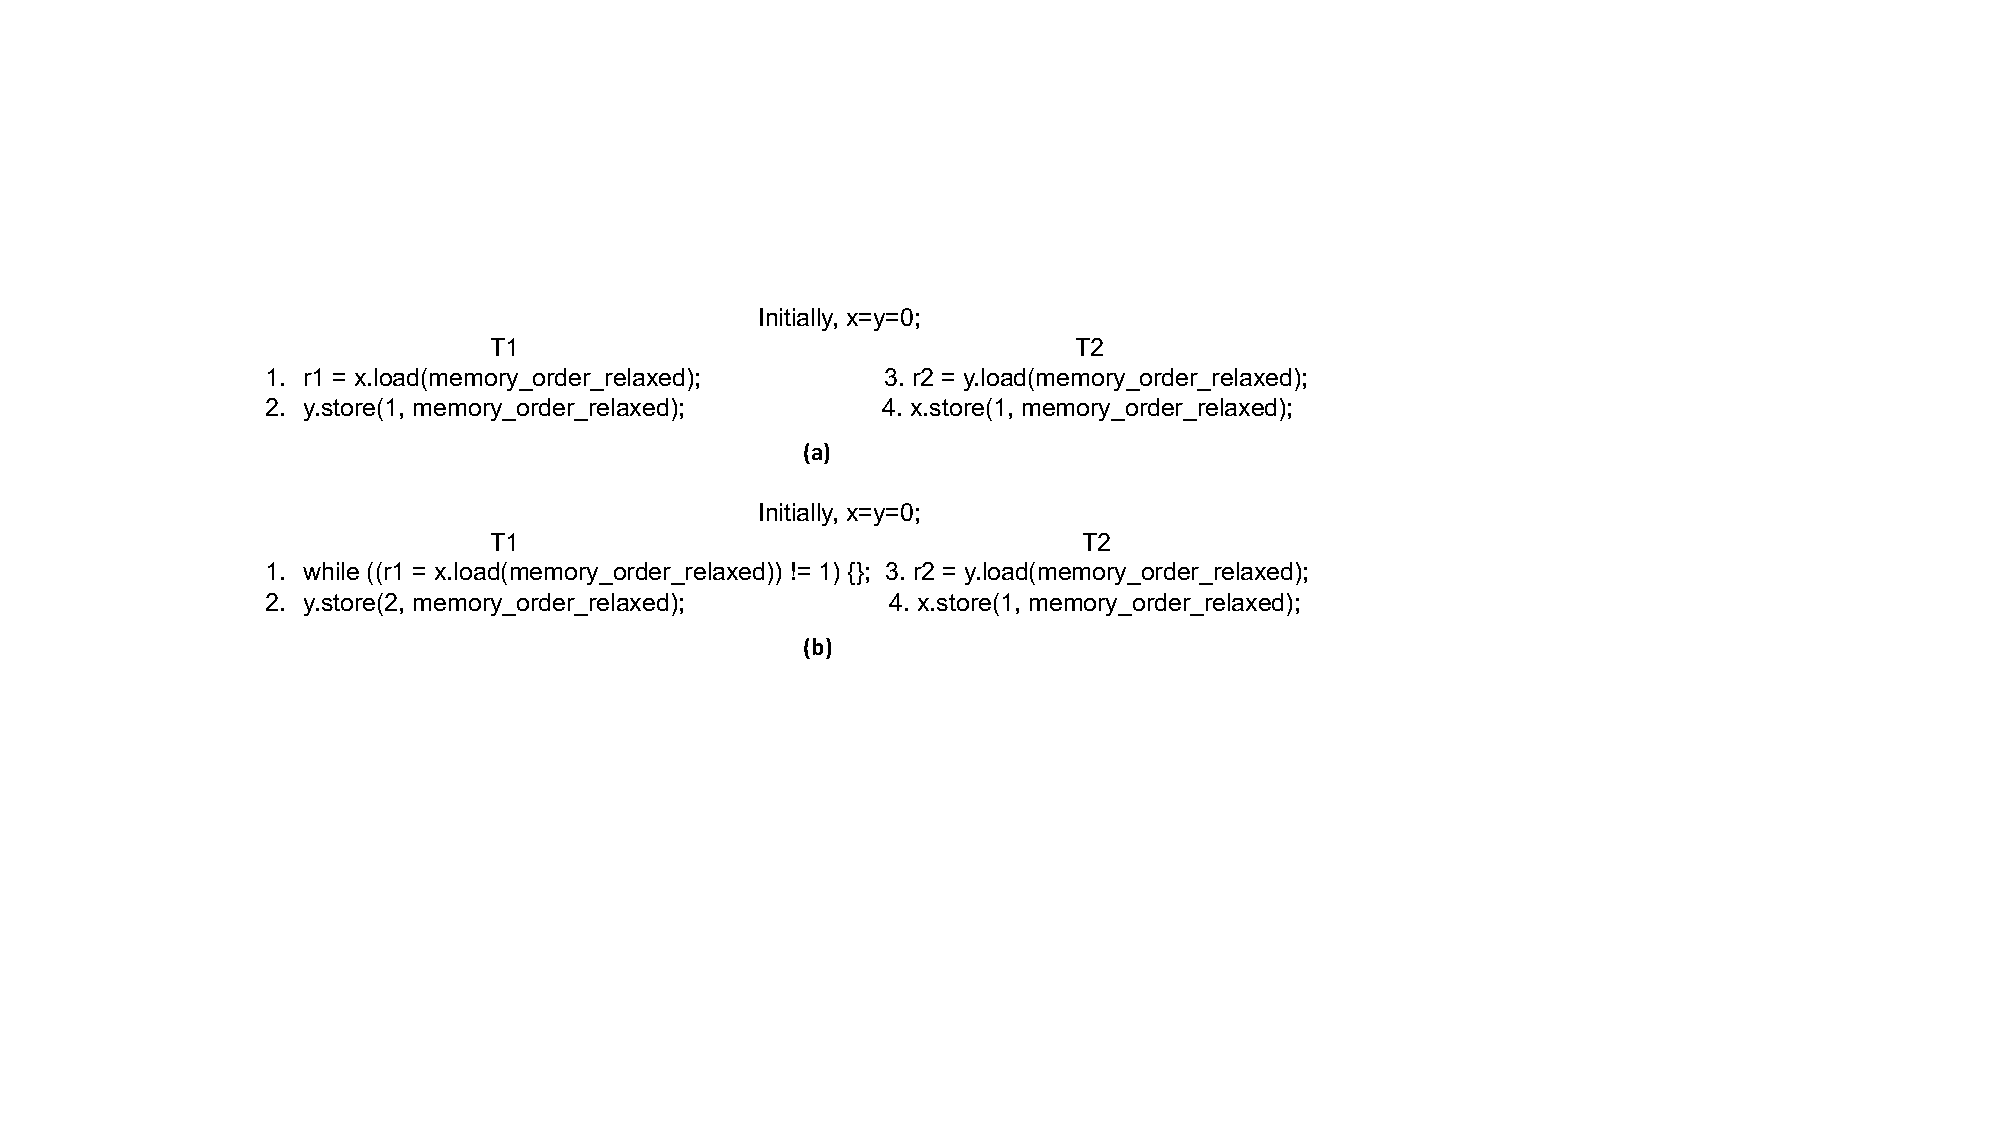
\includegraphics[scale=0.45]{soundnessCompleteness.pdf} %[width=6in]
\caption{Two simple examples for describing the soundness and completeness for
generating seeding interleavings.}
\label{fig:soundComplete}
\end{figure}

The most straightforward way of generating seeding interleavings is to iterate on each read $r$ 
in each thread and each possible value $v$ that $r$ may read and 
then generate a corresponding interleaving to enforce $r$ read $v$. 
However, this approach may generate redundant seed interleavings and thus harm the completeness. 

\begin{figure}%[t]
\centering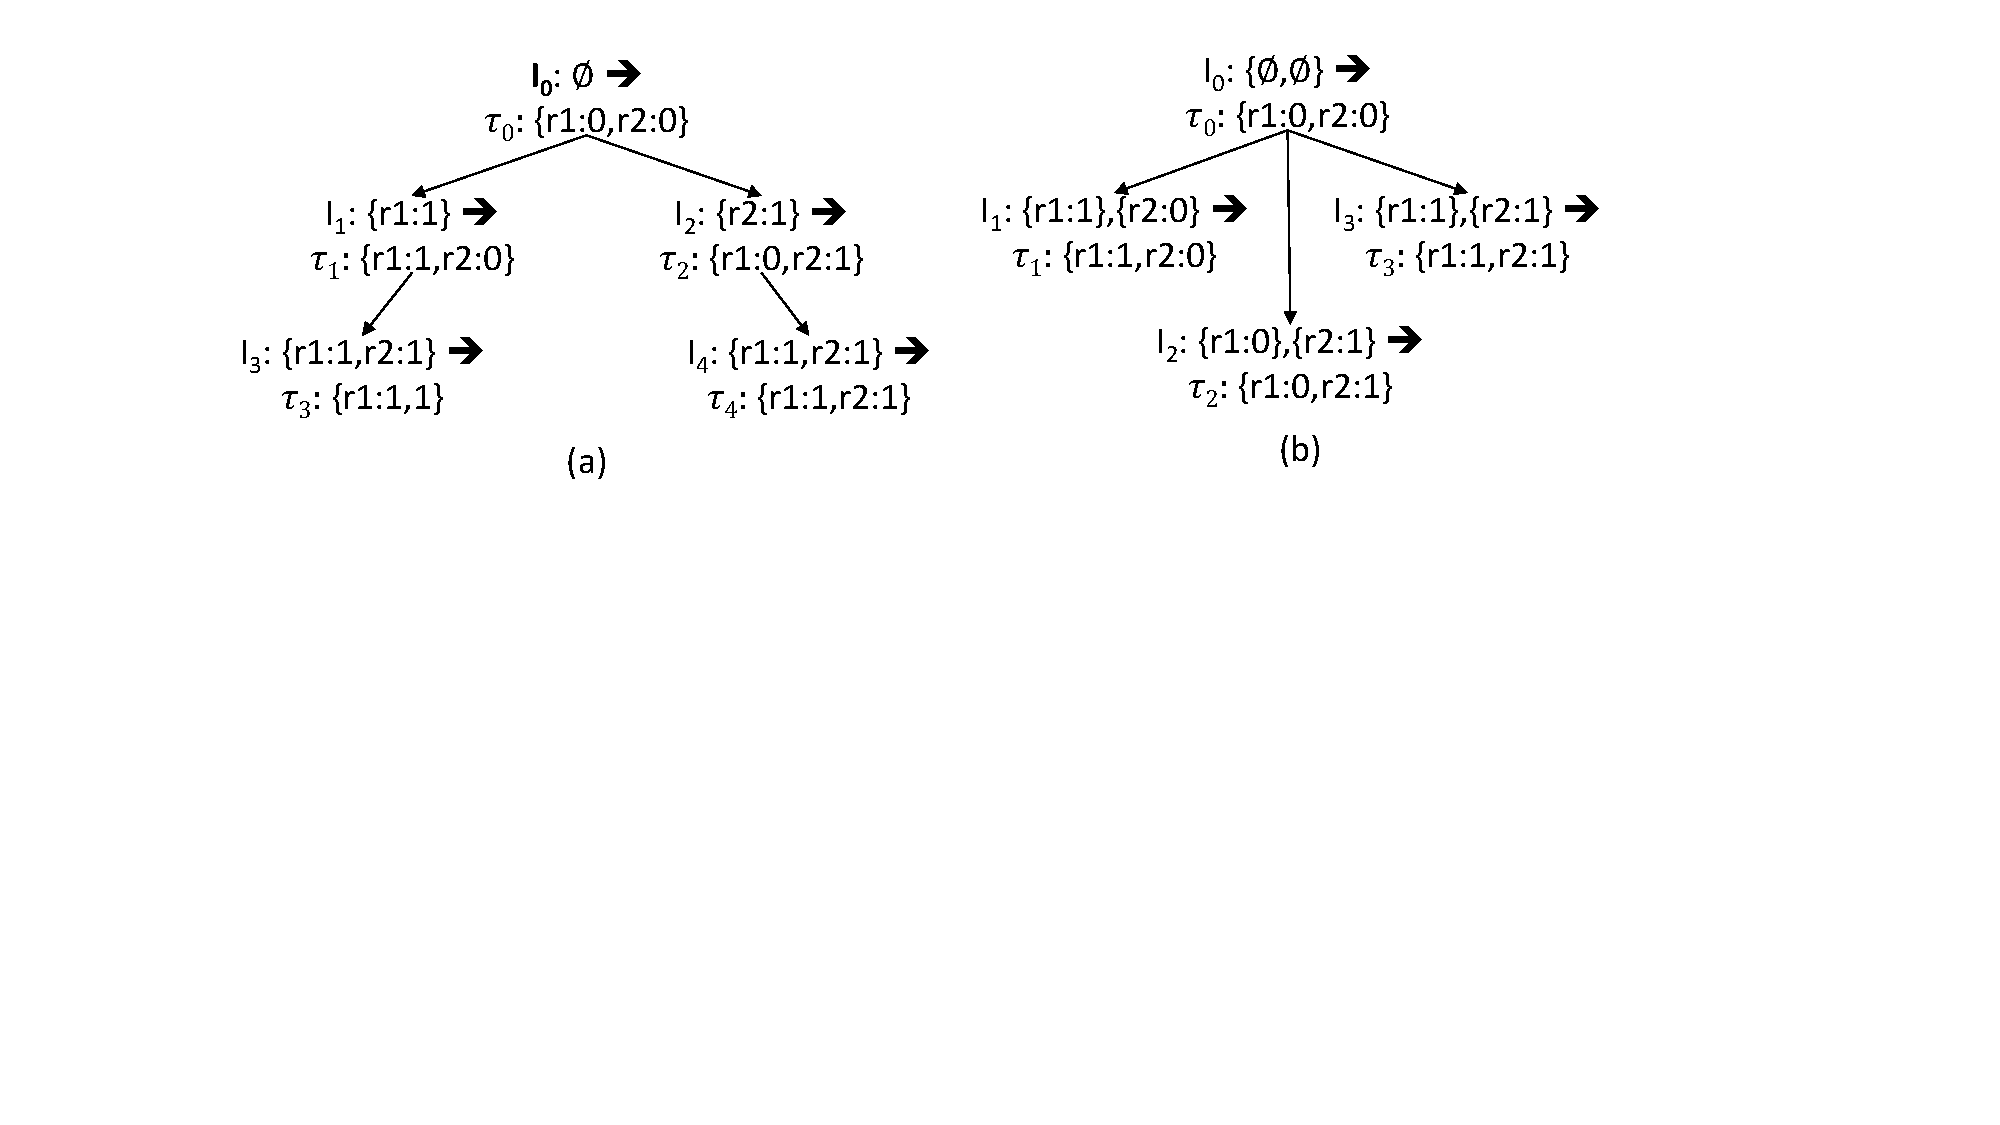
\includegraphics[scale=0.35]{interleavingGen.pdf} %[width=6in]
\caption{Two simple examples for describing the soundness and completeness for
generating seeding interleavings.}
\label{fig:interleavingGen}
\end{figure}

Take the code snippet in Figure~\ref{fig:soundComplete}(a) as example. Figure~\ref{fig:interleavingGen}(a)
describes the process of generating seed interleavings for exploring the whole search space by the straightforward
approach, starting with the initial empty seed interleaving $I_0$, which means no read is required to read a special value. 
Let $r$:$v$ represent read $r$ reading value $v$.
It ends with exploring five interleavings but only four different traces are explored, 
since trace $\{r1$:$1, r2$:$1\}$ is considered twice by both $I_3$ and $I_4$.
Note that the number of the redundant seed interleavings introduced by this approach will be \textit{exponential}
to that of reads along the trace. 

\subsection{Basic Algorithm}

This section will present the basic algorithm for generating seed interleavings to maintain 
both the completeness and soundness.

\begin{algorithm}%[t]
  \caption{{\bf IdentifyNewSch($\tau$)}}
%  its cycles as potential deadlocks.}}%: The top algorithm.
  \label{alg:gen}
{%\footnotesize
\begin{algorithmic}[1]
  \State{\Ind{0} \textbf{Input:} an input trace $\tau$;}
  \State{\Ind{0} \textbf{Output:} S - a set of new seed interleavings;}
  \State{\Ind{0} {\textit{// **For completeness**}}}
  \State{\Ind{0} {\bf for} (each $p\in allPrefixes(\tau)$)}
  \State{\Ind{1} {		\bf for} (each $v\in allValues(prefix)$)}
  \State{\Ind{2} {			\bf if} {$p$ reads $v$} as in $\tau$} {\bf then} continue;
  \State{\Ind{2} {			$\Phi_{rw}'(p, v) = \bigwedge_{\forall r\in prefix}\Phi_{rw}(r, vSet(r))$;}}
  \State{\Ind{2} {			$\Phi_{seed}(p,v)=\Phi_{hb}\wedge\Phi_{rw}'(p,v)\wedge\Phi_{co}$;}}
  \State{\Ind{2} {			$s\leftarrow$solve($\Phi_{seed}(p,v)$);}}
  \State{\Ind{2} {			\bf if ($s\neq null$)}} {\bf then} $S.add(s)$;
  \State{\Ind{2} {			\bf else}} $recheckList.add((p, v))$;
%  \State{\Ind{2} {			\bf end if}}
  \State{\Ind{1} {		\bf end for}}
  \State{\Ind{0} {\bf end for}}
  \State{\Ind{0} {\textit{// **For soundness**}}}
  \State{\Ind{0} {\bf for} (each pair $(p, v)\in recheckList$)}
  \State{\Ind{1} {		construct $\Phi_{seed}(p,v)$} as line 6$\sim$7;}
  \State{\Ind{1} {		$s\leftarrow$solve($\Phi_{seed}(p,v)$);}}
  \State{\Ind{1} {		\bf if ($s\neq null$)}} {\bf then} 
  \State{\Ind{2} {		$S.add(s)$; }}
  \State{\Ind{2} {		$recheckList.erase((p, v))$;}}
  \State{\Ind{0} {\bf end for}}
\end{algorithmic}
}
\end{algorithm}

\paragraph{Completeness}
To avoid such redundancy, we propose an approach based on
\textit{prefix combination}. As described in Algorithm~\ref{alg:gen}, when generating seed interleavings based on
the input trace $\tau$, we catch all prefixes exposed by $\tau$, as described by set $allPrefix(\tau)$, and then iterate
each prefix $p$ in the outer loop (between line 4 to 13). 
Specifically, $p=\{p_1,...,p_N\}$ contains a sub-prefix $p_i$ along the $i$-th thread, where $N$ represents 
the number of threads. Thus, there are $\prod_{1\leq i\leq N}|p_i|$ different prefixes for $p$.
For each $p$, it identifies all possible value combinations
that the reads in $p$ may read, represented by the set $allValues(p)$, which contains
$\prod_{r_i\in prefix}n_i(r_i)$ elements, where $n_i(r_i)$ is the number of different values that $r_i$
in $p$ can read. The inner loop (between line 5 to 12) iterates on each element
$v$ and tries to generate a new seed interleaving. 
Specifically, it constructs the formula $\Phi_{seed}(p,v)$ at line 8 to generate a consistent seed interleaving which 
enforce the reads in $p$ read the values described by $v$, as described by constraints $\Phi_{rw}'(p,v)$.
If $\Phi_{seed}(p,v)$ is solvable, then a new schedule is generated to trigger an execution which will explore new unexplored behavior.
Note that, the value combination that is just explored by the input trace will be skipped at line 6. 

For the code in Figure~\ref{fig:soundComplete}(a), our approach generates three seed interleavings ($I_1$ to $I_3$)
at the same time, as described in Figure~\ref{fig:interleavingGen}(b), and ends without any redundant executions.

\paragraph{Soundness}

While the loop iteration in Algorithm~\ref{alg:gen} maintains the completeness of the algorithm, it may miss some
consistent executions. Take the code snippet in Figure~\ref{fig:soundComplete}(b) as example. 
Suppose the initial trace is $\tau_0$: $\{r1$:$1,r3$:$2\}$, then prefix $p=\{r1$:$0,r3$:$2\}$ will be 
identified as an unreachable prefix based on $\tau_0$, because when $r1$ reads value $0$ then the reachability of 
the write at line 2 will not be guaranteed and thus $r2$ can not read value $2$. However, $p$ is actually reachable
and contains a more concrete prefix $\{r1$:$0,r2$:$1,r3$:$2\}$.

For the soundness, Algorithm~\ref{alg:gen} maintains the currently discovered unreachable prefixes in set $recheckList$,
and rechecks their reachability when a new trace is generated, as described by the loop between line 15 and 21.
$reCheckList$ is updated at line 20 whenever a pair $(p,v)$ is successfully identified as a reachable prefix by a seed interleaving.
Take prefix $p=\{r1$:$0,r3$:$2\}$ as example. It is added to $recheckList$ when identified, and will be checked and satisfied
when new trace $\tau'$: $\{r1$:$0,r2$:$1,r3$:$0\}$ is triggered by the seed interleaving 
corresponding to the prefix $p'=\{r1$:$0,r3$:$0\}$ generated base on $\tau_0$.

\begin{theorem}
Suppose the program is terminating and the solver is sound (i.e, for a satisfiable constraint formula
 the solver will always return a correct solution), our approach will eventually cover the whole state-space
of the program that can be driven by the possible interleavings with respect to a given input.
\end{theorem}

\textit{Proof.} \textit{By contradiction}. Suppose there exists an interleaving $I$ is not covered, and 
$I$ will explore the behavior that the explored interleavings do not touch.
Two possibilities exist: (1) $I$ contains an previously observed read which reads a new unobserved value;
(2) $I$ contains a previously unobserved event. 
Obviously, case (1) is impossible, because our algorithm consider all possible values that a read event can read.
For case (2), whenever a new trace is observed, our algorithm consider all prefixes exposed by the given input trace. 
Thus, an event is not considered only when it dependents on a branch, the condition of which can not be satisfied by any 
of the states driven by the generated seed interleavings. However, it contradicts to the fact that our algorithm
generates a seed interleaving for each possible value set that the reads in a prefix can read.

\subsection{Handle Nonterminating Programs}

Many realistic concurrent programs are nonterminating and thus have cyclic state spaces~\cite{Musuvathi:2008}.
Specifically, infinite spaces of executions exist for these programs when allowed to continually read 
the same value from an atomic object (even after new values have been written to the
object). Take Figure~\ref{fig:soundComplete}(b) as example. If line 1 continues to read the initial value $0$, 
then thread $T1$ will not terminate and thus introduce an infinite search space. 

To handle such nonterminating programs, we introduce two strategies. 
First, \checker supports CHESS-like~\cite{Musuvathi:2008}
fairness based the thread-\textit{yield} statements in the test programs. 
This strategy can efficiently prevent the nontermination resulted from unfair schedules.
Second, \checker supports a user-defined number to limit the times that
the same value from an atomic object can be continually read. 
During the seed interleaving generation, \checker can use this number to 
generate fair schedules without tripping into a circle state space.

\section{Evaluation}

To evaluate our approach, we have developed a stateless model checker, called \checker,
which is implemented as a shared library to handles the 
atomic operations. Specifically, based compiler architecture LLVM~\cite{Lattner:2004}, we firstly compile
the tested programs into LLVM Bitcode, which contains a fixed number of atomic operations,
and then replace the atomic operations in the bitcode to the corresponding calls in the shared 
library to totally control their executions based on a given seed interleaving. 

Since C++11 is new, only few tools supports C++11 memory model and few benchmarks are available. 
Some existing tools are designed for different purpose, and thus have limitations on scalability 
(only considering small programs) or soundness (missing many potential program behavior). 
In this paper, we will mainly compare \checker with CDSChecker~\cite{Norris:2013}, which is the most
recently publicly available tool for C++11. 
We compiled our evaluations with compiler Clang's $-O3$ optimization, and ran all our experiments 
on a four-core machine with 2.70GHz Intel Core i5 CPU 703 running Ubuntu 14.04, 
and set a timeout of one hour for each benchmark.


%\appendix
%\section{Appendix Title}

%This is the text of the appendix, if you need one.

%\acks
%Acknowledgments, if needed.

% We recommend abbrvnat bibliography style.

\bibliographystyle{abbrvnat}
\bibliography{references}
% The bibliography should be embedded for final submission.

%\begin{thebibliography}{}
%\softraggedright
%\end{thebibliography}











\end{document}
